%%%%%%%%%%%%%%%%%%%%%%%%%%%%%%%%%%%%%%%%%%%%%%%%%%%%%%%%%%%%%%%%%%%%
%% I, the copyright holder of this work, release this work into the
%% public domain. This applies worldwide. In some countries this may
%% not be legally possible; if so: I grant anyone the right to use
%% this work for any purpose, without any conditions, unless such
%% conditions are required by law.
%%%%%%%%%%%%%%%%%%%%%%%%%%%%%%%%%%%%%%%%%%%%%%%%%%%%%%%%%%%%%%%%%%%%

\documentclass[
  digital, %% This option enables the default options for the
           %% printed version of a document. Replace with `digital`
           %% to enable the default options for the digital version
           %% of a document.
  table,   %% Causes the coloring of tables. Replace with `notable`
           %% to restore plain tables.
  lof,     %% Prints the List of Figures. Replace with `nolof` to
           %% hide the List of Figures.
  nolot,   %% Prints the List of Tables. Replace with `nolot` to
           %% hide the List of Tables.
  nocover
  %% More options are listed in the user guide at
  %% <http://mirrors.ctan.org/macros/latex/contrib/fithesis/guide/mu/fi.pdf>.
]{fithesis3}

%% The following section sets up the locales used in the thesis.
\usepackage[
  main=slovak, %% By using `czech` or `slovak` as the main locale
               %% instead of `english`, you can typeset the thesis
               %% in either Czech or Slovak, respectively.
  slovak, english %% The additional keys allow
]{babel}          %% foreign texts to be typeset as follows:
				  %%  \begin{otherlanguage}{english}  ... \end{otherlanguage}

\usepackage{paratype}

%% The following section sets up the metadata of the thesis.
\thesissetup{
    date          = \the\year/\the\month/\the\day,
    university    = mu,
    faculty       = fi,
    type          = mgr,
    author        = Matej Majdiš,
    gender        = m,
    advisor       = doc. RNDr. Vlastislav Dohnal\, Ph.D.,
    title         = {Rozpoznanie užívateľa na základe informácií o HTTP komunikácií},
    TeXtitle      = {Rozpoznanie užívateľa na základe informácií o HTTP komunikácií},
    keywords      = {keyword1, keyword2, ...},
    TeXkeywords   = {keyword1, keyword2, \ldots},
    assignment  = {} %TODO - prnted - Kopie zadání a Kopie prohlášení autora školního díla
}

\thesislong{abstract}{
	TODO
}

%TODO - printed - poďakovanie
%\thesislong{thanks}{ 
%	TODO
%}

%% The following section sets up the bibliography.
\usepackage{csquotes}
\usepackage[              %% When typesetting the bibliography, the
  backend=biber,          %% `numeric` style will be used for the
  style=numeric,          %% entries and the `numeric-comp` style
  citestyle=numeric-comp, %% for the references to the entries. The
  sorting=none,           %% entries will be sorted in cite order.
  sortlocale=auto         %% For more unformation about the available
]{biblatex}               %% `style`s and `citestyles`, see:
%% <http://mirrors.ctan.org/macros/latex/contrib/biblatex/doc/biblatex.pdf>.
\addbibresource{example.bib} %% The bibliograpic database within
                          %% the file `example.bib` will be used.
                          
\usepackage{makeidx}      %% The `makeidx` package contains
\makeindex                %% helper commands for index typesetting.

%% These additional packages are used within the document:
\usepackage{paralist}
\usepackage{amsmath}
\usepackage{amsthm}
\usepackage{amsfonts}
\usepackage{url}
\usepackage{menukeys}
\usepackage{float}
\usepackage[plainpages=false, pdfpagelabels]{hyperref}
\usepackage{listings}
\usepackage{color}
 
\definecolor{codeblue}{rgb}{0,0,0.6}
\definecolor{codegray}{rgb}{0.5,0.5,0.5}
\definecolor{codepurple}{rgb}{0.58,0,0.82}

\lstdefinestyle{mystyle}{  
    commentstyle=\color{codegray},
    keywordstyle=\color{codeblue},
    numberstyle=\tiny\color{codepurple},
    stringstyle=\color{codepurple},
    basicstyle=\footnotesize
}
 
\lstset{style=mystyle}

\begin{document}

\chapter{Úvod}
Problematika jednoznačnej identifikácie používateľa je dnes veľmi
dôležitou a riešenou témou. Jedným z hlavných dôvodov je fakt, že väčšina
dnešných existujúcich, prípadne novo vznikajúcich systémov a aplikácií, je
nejakým spôsobom zapojená do Internetu. 

Z toho vyplýva potreba rozoznania a identifikácie používateľov, ktorí s
danou aplikáciou interagujú. Existuje niekoľko rôznych prístupov k 
identifikácii, od mapovania IP adries sieťovej vrstvy až po aplikačnú správu
užívateľských účtov. Každý z nich má však svoje výhody aj nevýhody. Podrobne sa nimi zaoberá kapitola \ref{ch:existing}.

Cieľom práce je vytvoriť unikátny identifikátor na základe informácií
dostupných najmä z \textit{HTTP}, prípadne \textit{TCP} protokolu. Pred zostavením samotného algoritmu je
však dôležité popísať niektoré kľúčové oblasti a postupy.
Nasledujúce odseky úvodu práce sa preto budú stručne zaoberať fungovaním aplikácií typu
klient-server a architektúrou domény práce. 

\section{Aplikácie typu Klient-Server}
S pokračujúcim vývojom nových technológií sa Internet a Web stávajú čoraz väčšou
súčasťou našich životov. Web ako taký už dávno nie je limitovaný prehliadaním na
počítačoch. Musí sa prispôsobovať rôznym technológiám, ako sú napríklad
mobilné, či iné multimediálne zariadenia.

Najčastejšie používaným modelom sieťovej komunikácie pre
architektúru aplikácií je takzvaný klient-server model. Základnou
myšlienkou tohto modelu je zaslanie požiadavky (\textit{requestu}) klientom na
server, ktorý vystupuje ako poskytovateľ služby.

\subsection{Klient-Server model}
Pretože Klient-Server model je používaný rôznymi typmi aplikácií, bolo nutné
použiť štandardizované protokoly, na základe ktorých bude možné komunikovať.
Niektorými z najpoužívanejších protokolov sú: \textit{FTP (File Transfer Protocol)},
\textit{Simple Mail Transfer Protocol (SMTP)} a \textit{Hypertext Transfer
Protocol (HTTP)}. Bližšie sieťové vrstvy a jednotlivé protokoly popisuje
kapitola \ref{ch:net-layers}.

\begin{figure}[h]
  \centering
    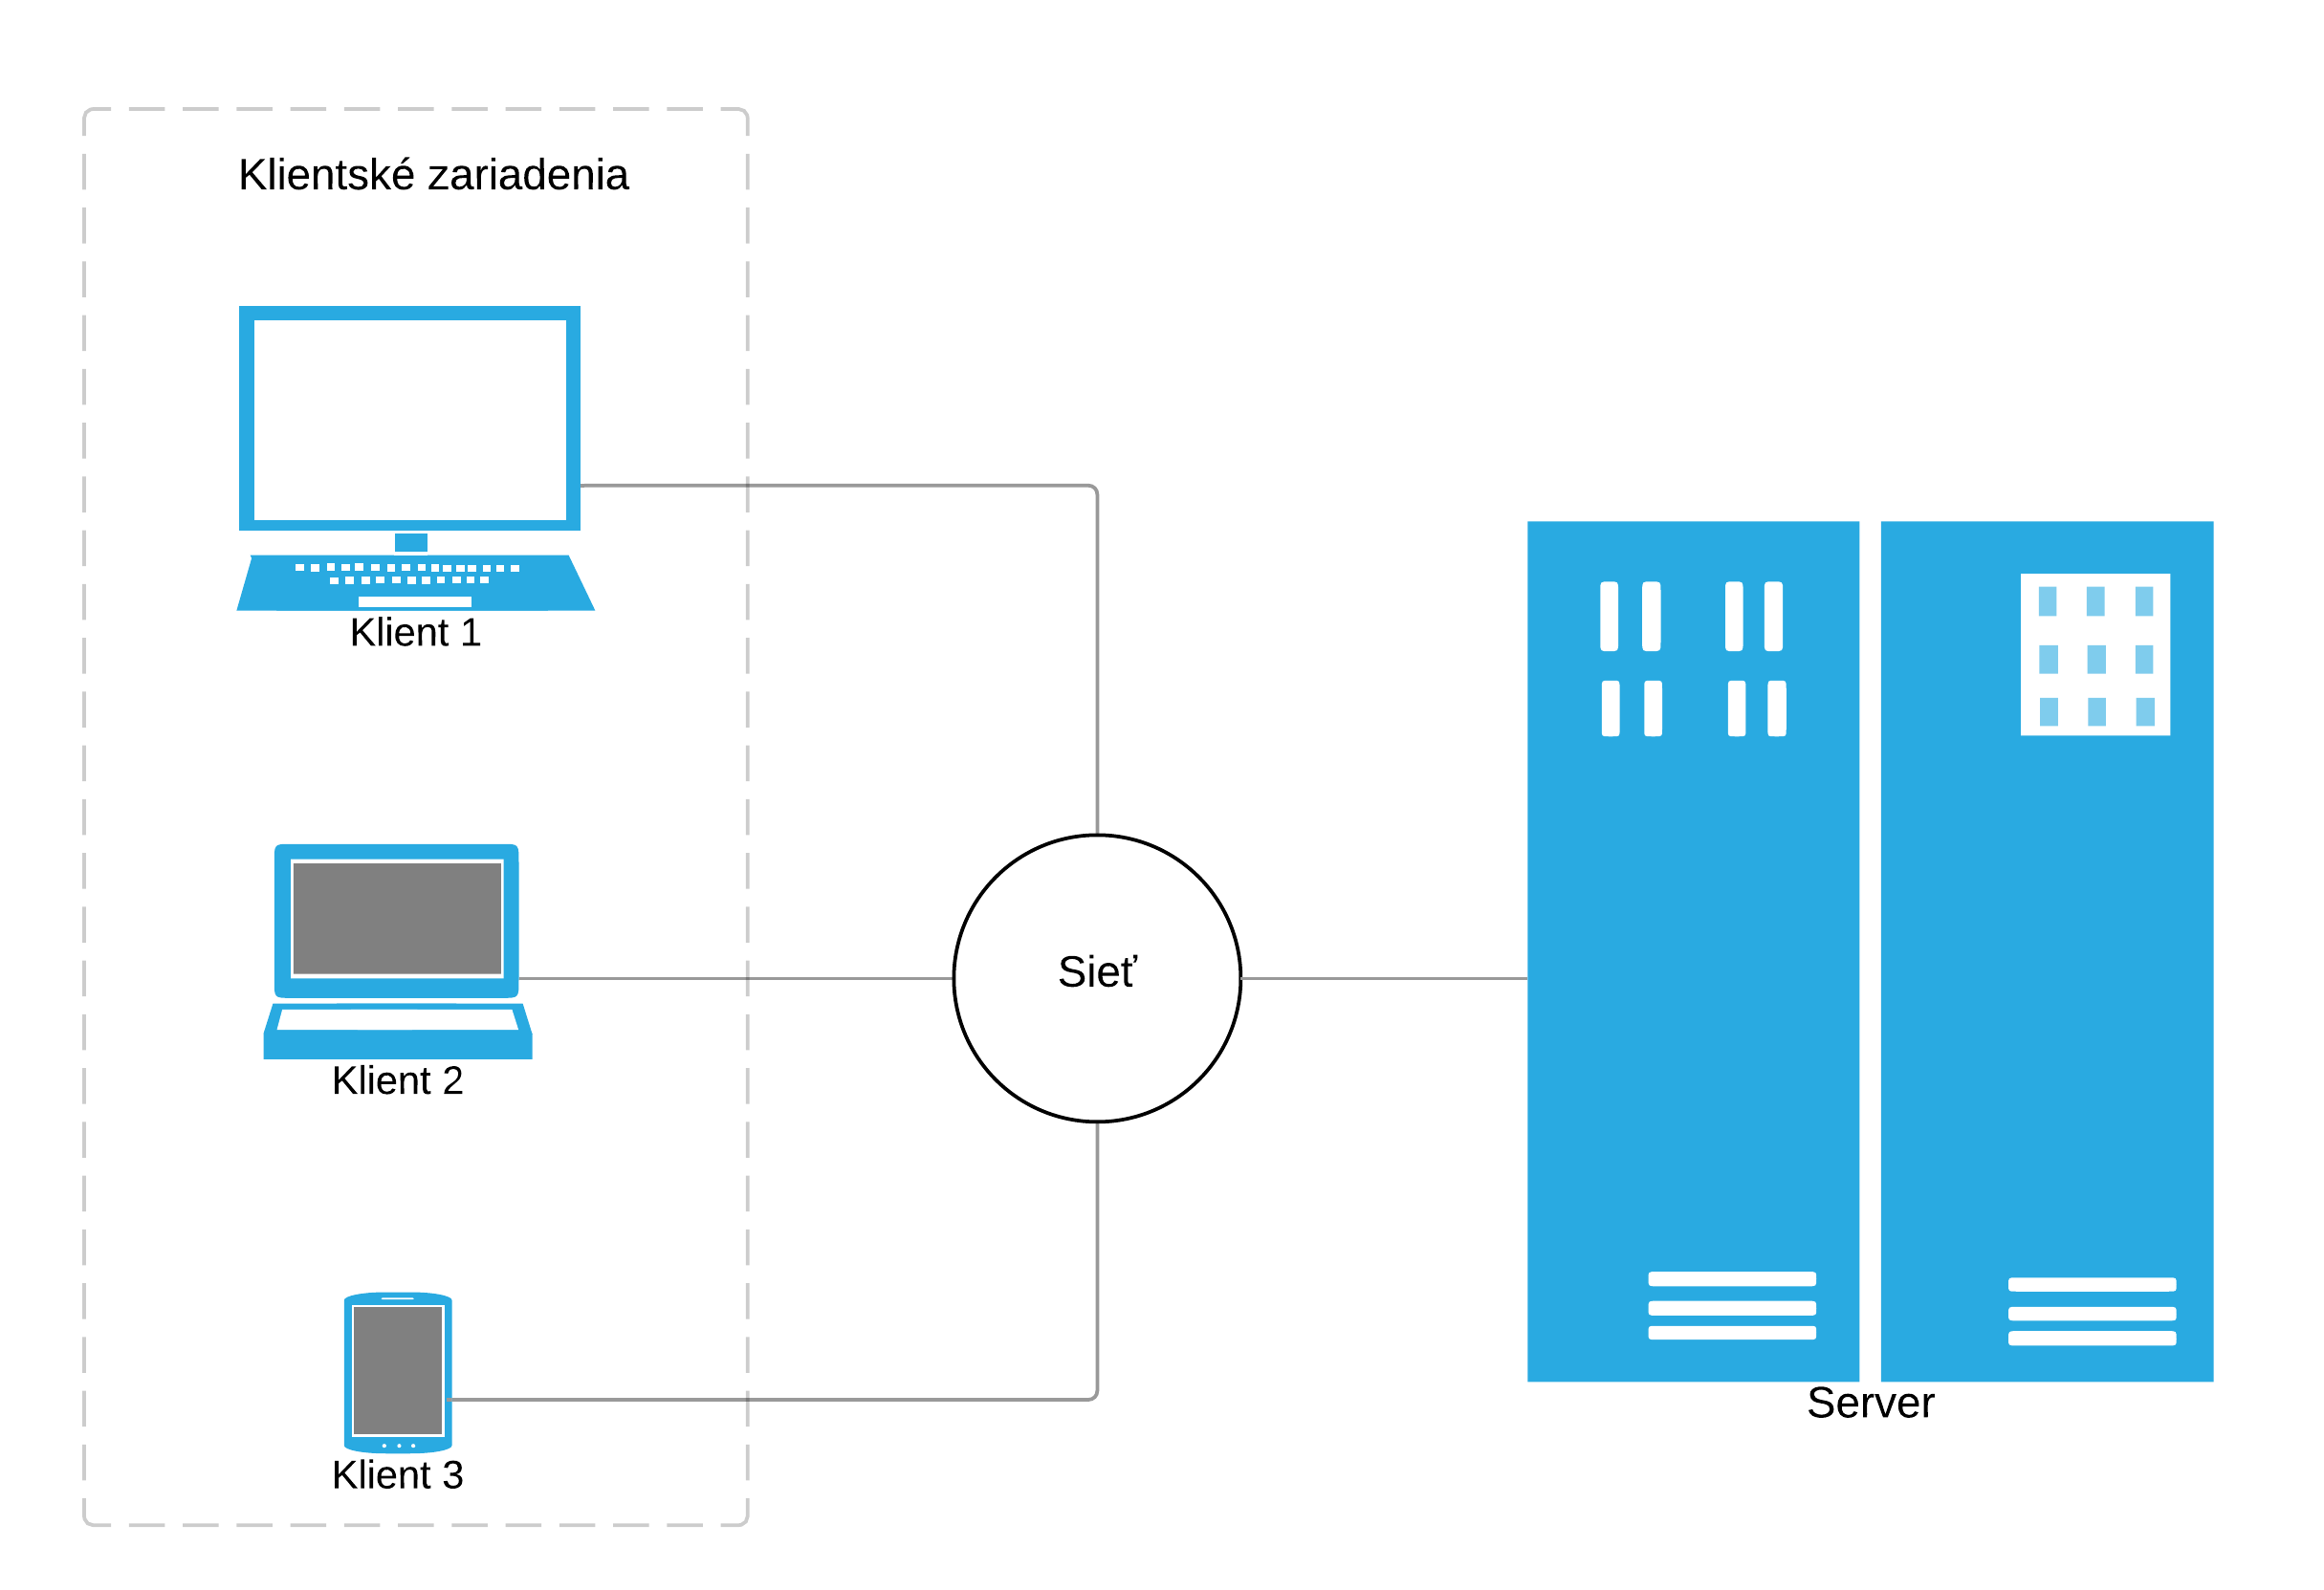
\includegraphics[width=.94\textwidth]{images/C-S-basic.png}
  \caption{Schéma znázorňuje základnú architektúru modelu Klient-Server, zdroj:
  vlastné spracovanie}
  \label{fig:cs-basic}
\end{figure}

\subsection{Architektúra}
Architektúra klient-server modelu sa vo všeobecnosti typicky skladá z troch 
častí:
\begin{itemize}
	\item Aplikačný server
	\item Databázový server
	\item Zariadenie klienta
\end{itemize}
Zároveň existujú dva základné typy architektúr podľa miery zapojenia zariadenia klienta: 
\begin{itemize}
	\item 2-stupňová \textit{(2-tier)}
	\item 3-stupňová \textit{(3-tier)}
\end{itemize}

\begin{figure}[H]
  \centering
    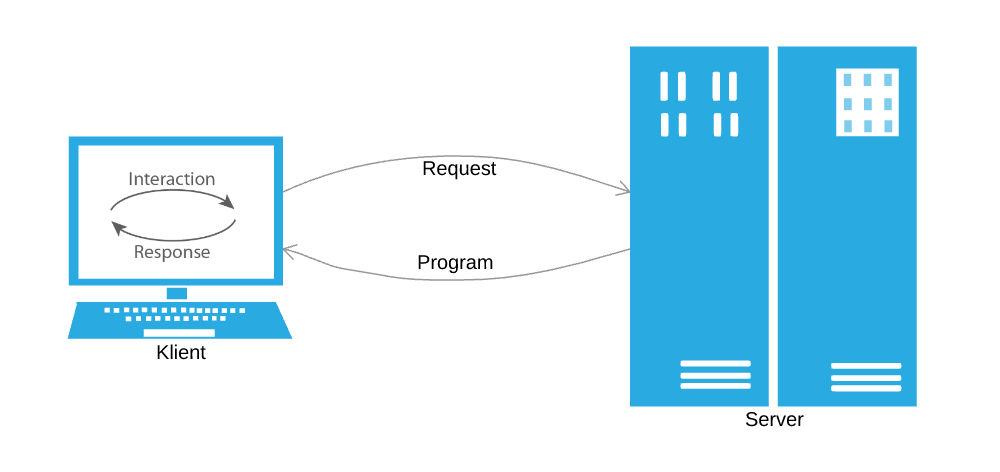
\includegraphics[width=.82\textwidth]{images/C-S-thick.png}
  \caption{Grafické znázornenie a popis priebehu komunikácie 2-tier architektúry,
  zdroj: vlastné spracovanie}
  \label{fig:cs-thick}
\end{figure}

\textit{2-tier} architektúra zahŕňa len zariadenie klienta a databázový server.
U tohoto typu architektúry je aplikácia spustená na zariadení klienta, ktoré sa
následne pripája priamo na server. Zariadenie tak obsluhuje zároveň
\textit{business} logiku aj zobrazovanie aplikácie. Tento typ architektúry
nazývame aj tučný klient (\textit{thick client}).

\begin{figure}[H]
  \centering
    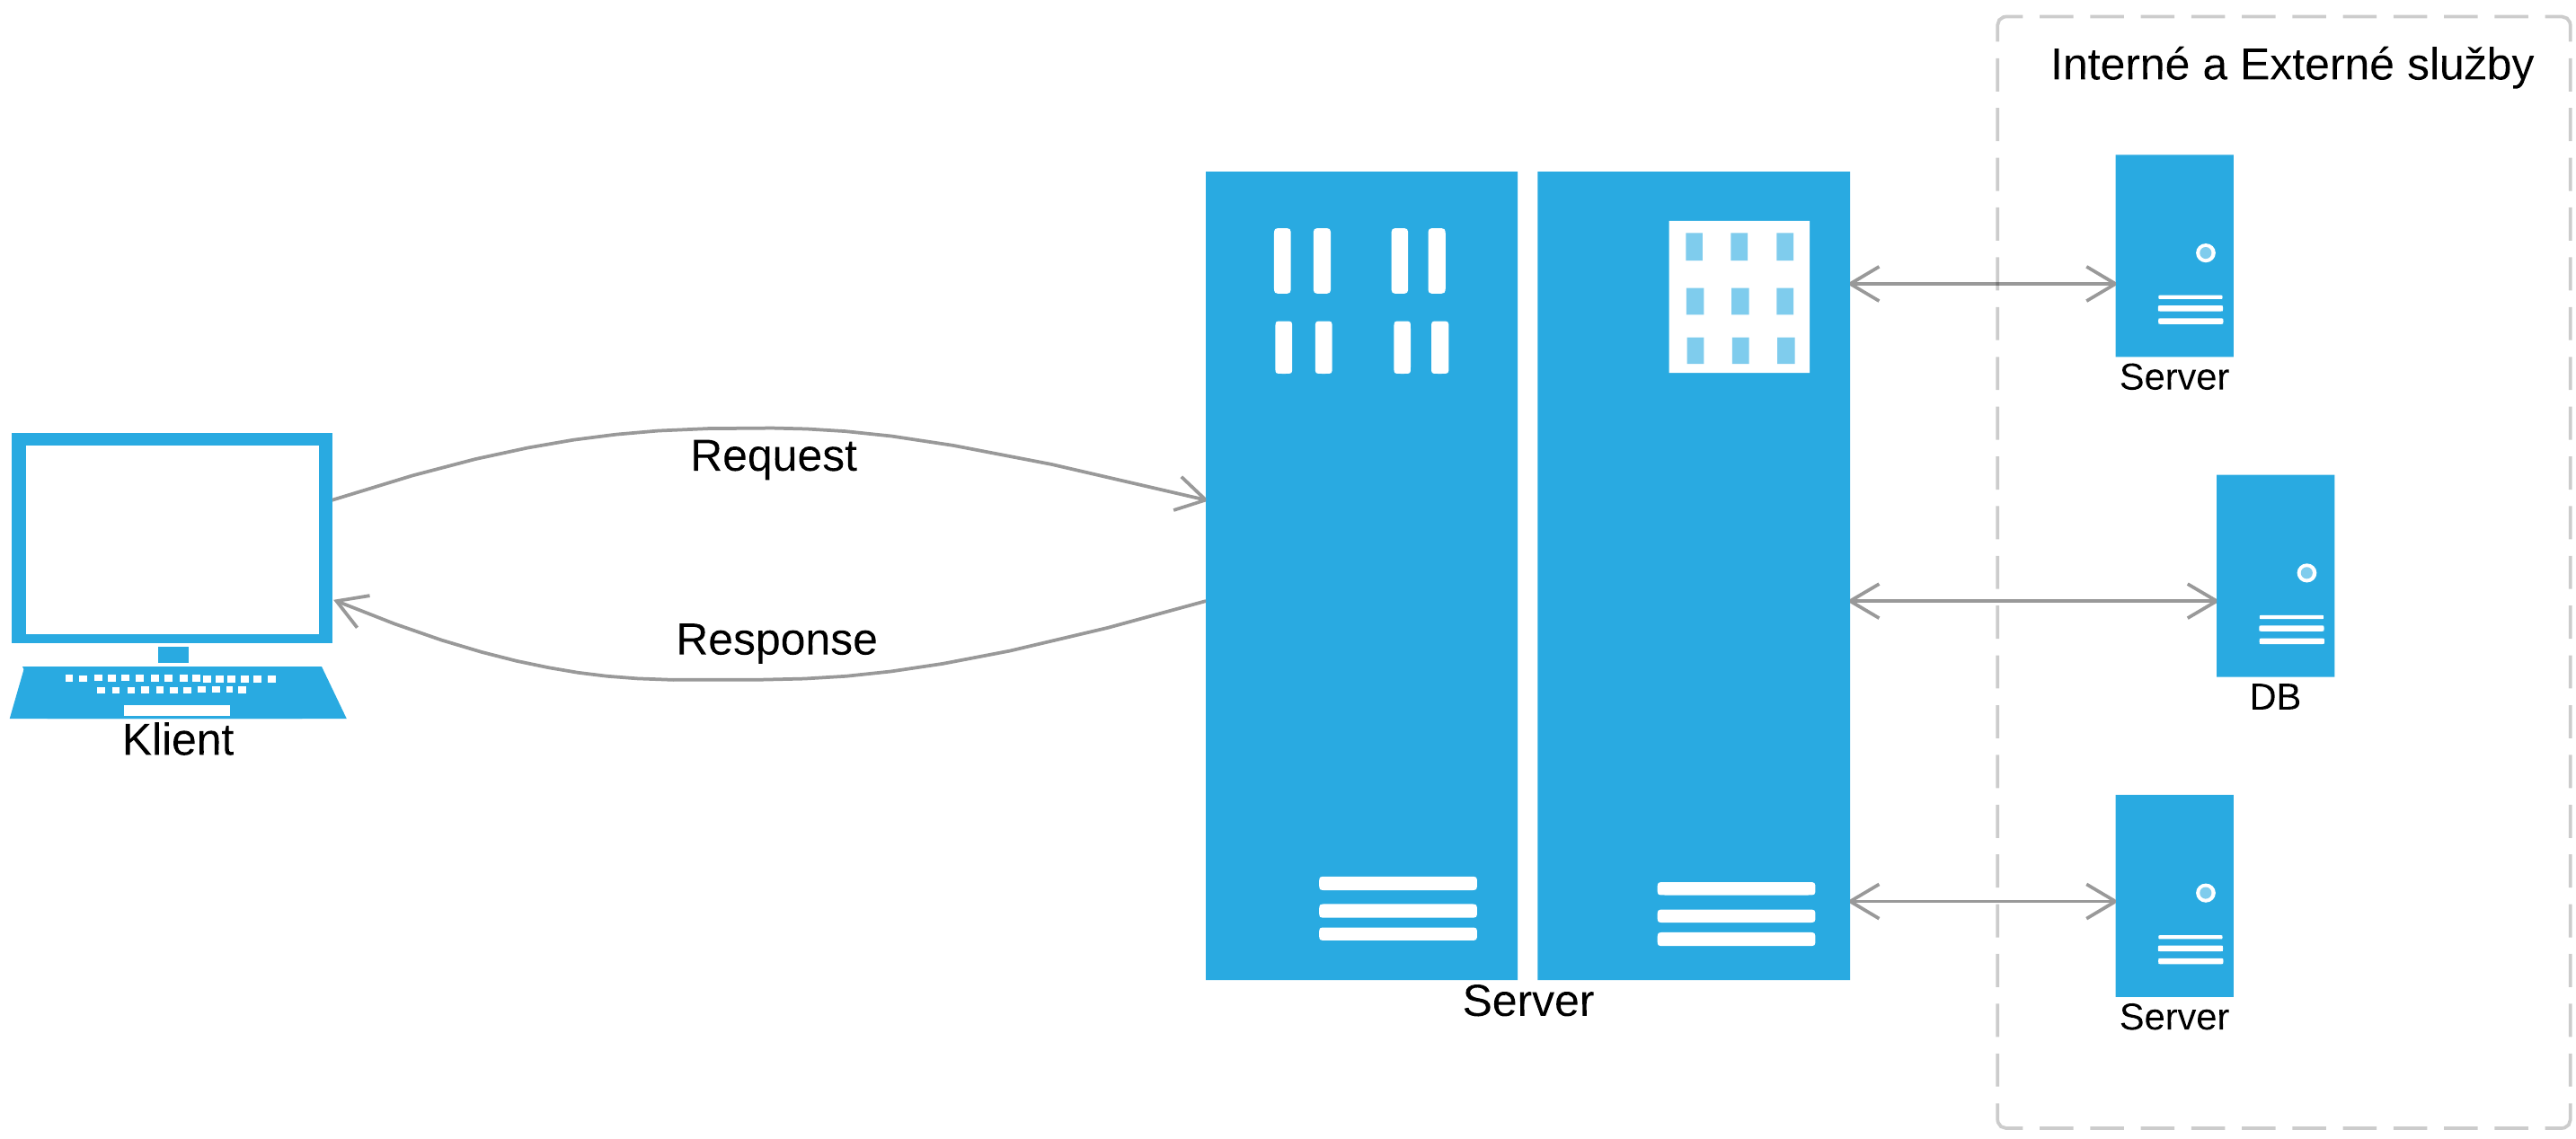
\includegraphics[width=\textwidth]{images/C-S-thin.png}
  \caption{Grafické znázornenie a popis priebehu komunikácie 3-tier architektúry,
  zdroj: vlastné spracovanie}
  \label{fig:cs-thin}
\end{figure}

\textit{3-tier} architektúra, ktorej aplikácie sú predmetom tejto práce, sa od
\textit{2-tier} líši najmä tým, že okrem zariadenia klienta a databázového serveru,
zahŕňa aj aplikačný server. Tento je následne používaný na obsluhu
\textit{business} logiky aplikácie a komunikáciu s databázou, pričom zariadenie
klienta slúži len na zobrazovanie. Iný názov pre takýto typ architektúry je tenký
klient (\textit{thin client}).

\section{Štruktúra práce}
Práca je ďalej rozdelená na dve časti, pozostávajúce z piatich kapitol, z ktorých každá sa zaoberá iným aspektom
jej charakteristiky:
\begin{itemize}
\item Prvá časť práce sa zameriava na
definíciu dôležitých pojmov, popis použitých technológií a porovnanie existujúcich prístupov k identifikácii.
\item Druhá časť sa venuje samotnému návrhu algoritmu identifikátora, jeho implementácií a testovaniu jeho funkcionality.
\end{itemize}

Najskôr teda kapitola
\ref{ch:net-layers} popisuje jednotlivé sieťové vrstvy a protokoly, ktorých
informácie bude možné následne použiť k tvorbe identifikátora. 
Nasleduje kapitola \ref{ch:dos} popisujúca hlavnú z motivácií 
celej práce, ktorou sú útoky typu DOS a prevencia voči nim.
Posledná kapitola prvej časti práce je zhrnutím
existujúcich prístupov k rozpoznaniu užívateľov v kapitole \ref{ch:existing}.

Najdôležitejšou časťou sú však
samozrejme kapitoly \ref{ch:footprint} a \ref{ch:data}, ktoré popisujú návrh samotného 
algoritmu identifikátora, jeho implementáciu a následné testovanie s reálnymi dátami.

\chapter{Sieťové vrstvy}
\label{ch:net-layers}
Pre lepšie uchopenie problematiky identifikácie používateľa je nutné najskôr
popísať jednotlivé sieťové vrstvy TCP/IP modelu a
ich protokoly. Nasledujúci text sa preto zameriava najmä na štruktúry, ktorých pochopenie je
dôležité pre ďalšie moduly teoretickej a praktickej časti práce. Ide teda o
konkrétne informácie jednotlivých protokolov, z ktorých niektoré boli následne použité v implementácií
identifikačného algoritmu.

\begin{figure}[h]
  \centering
    
\includegraphics[width=.99\textwidth]{images/net-layers.png}
  \caption{Vizualizácia vrstiev TCP/IP modelu, jeho najpoužívanejších protokolov
  a prenosových štruktúr, zdroj: vlastné spracovanie}
  \label{fig:net-layers}
\end{figure}

\section{Aplikačná vrstva}
Na vrchole hierarchie je Aplikačná vrstva abstrakciou, ktorá špecifikuje
konkrétne protokoly a metódy používané hostiteľskými uzlami v sieti. Táto
vrstva je definovaná jednak v TCP/IP, ale aj OSI
\textit{(Open Systems Interconnection)} modeli sieťovej komunikácie.

Táto práca narába s modelom TCP/IP, v ktorom aplikačná vrstva definuje práve
protokoly a metódy rozhraní pre komunikáciu medzi jednotlivými procesmi
spájaných strán v sieti. Samotná aplikačná vrstva však len štandardizuje formu
komunikácie, pričom ustálenie uceleného dátového spojenia a správu prenosu dát
u aplikácií typu klient-server a \textit{peer-to-peer} ponecháva na protokoloch
nasledujúcej - transportnej vrstvy. Keďže aplikačná vrstva nijakým spôsobom
nepopisuje a nešpecifikuje konkrétne pravidlá pre formu prenášaných dát,
aplikácie samotné musia obsahovať logiku, ktorá zabezpečí, že obe komunikujúce
strany budú v tomto ohľade navzájom kompatibilné.

Aplikačná vrstva definuje veľké množstvo používaných protokolov, ako napríklad:
\begin{itemize}
	\item HTTP/HTTPS
	\item TLS/SSL poskytujúci zabezpečenú vzdialenú komunikáciu po sieti
	\item FTP využívaný na prenos súborov
	\item SMTP určený pre emailovú komunikáciu
	\item DNS realizujúci systém hierarchie doménových mien, a iné...
\end{itemize}
Pri tvorbe identifikátora sa však budeme venovať najmä informáciám z protokolov
rodiny HTTP, konkrétne teda hlavičkám a atribútom HTTP a HTTPS.

\subsection{HTTP}
HTTP \textit{(Hypertext Transfer Protocol)} je distribuovaný protokol určený
na spoluprácu a prenos informácií medzi jednotlivými systémami pre
prácu s hypermédiami. Tento protokol je bezstavový a vo všeobecnosti
použiteľný nielen pre prenos hypertextu, ale aj správu DNS serverov, prípadne
zložitejších objektov a systémov, v ktorých uplatní rozsiahlu škálu svojich
hlavičiek a chybových hlášok. Jedným z jeho charakteristických znakov je aj
možnosť voľby reprezentácie dát, čo dáva systémom veľkú nezávislosť na
prenášanom formáte.

HTTP funguje na princípe požiadavky a odpovede \textit{(request - response)},
založenom na fungovaní samotného klient - server modelu. Klientom môže byť
napríklad webový prehliadač, serverom zasa aplikácia spustená na zariadení
hostiteľského uzlu. V tomto prípade teda webový prehliadač zašle správu vo
forme HTTP požiadavky na server. V ideálnom prípade server požiadavku
\textit{(request)} spracuje a vygeneruje odpoveď (napríklad HTML stránku),
ktorú vráti klientovi ako správu vo formáte HTTP odpovede \textit{(response)}.
Odpoveď pre klienta vždy obsahuje takzvaný \textit{(status)}, ktorý informuje o
dokončení požiadavky a prípadné telo so správou odpovede.

Celá relácia HTTP spojenia medzi dvoma uzlami je teda sekvenciou niekoľkých
takýchto \textit{(request - respone)} transakcií. Samotný prenos dát však nie
je realizovaný na úrovni HTTP protokolu, ale prostredníctvom protokolu TCP
na úrovni transportnej vrstvy. HTTP klient iniciuje ustálenie TCP spojenia pre
špecifický port serveru (typickými portami sú 80, 443 alebo 8080). HTTP server
počúva na danom porte a čaká na správu požiadavky klienta. Po prijatí správy ju
už server štandardne spracuje a vráti odpoveď. 

Klient a server komunikujú prostredníctvom zasielania textových správ.
Požiadavka pozostáva z nasledujúcich informácií: 
\begin{itemize}
	\item Definícia požiadavky
	\item HTTP hlavičky (napríklad: \textit{Accept-Language: en})
	\item Prázdny riadok
	\item Prípadné telo správy
\end{itemize}

Takisto správa odpovede má definovaný formát podobný formátu požiadavky, ktorý
sa skladá z nasledujúcich položiek:
\begin{itemize}
	\item Status spracovania požiadavky a dôvod
	\item HTTP hlavičky odpovede (napríklad: \textit{Content-Type: text/html})
	\item Prázdny riadok
	\item Prípadné telo správy odpovede
\end{itemize}

Prvý riadok definície a každá z hlavičiek musia byť zakončené znakmi
\textit{<CR><LF>}
(znak pre \textit{carriage return} nasledovaný znakom \textit{line feed}).
Prázdny riadok musí zároveň pozostávať výlučne zo znakov \textit{<CR><LF>}.
Z pohľadu identifikácie budú neskôr veľmi dôležité práve HTTP hlavičky. U HTTP
verzie 1.1 je jedinou povinnou hlavičkou \textit{Host} definujúci server, na
ktorý bola požiadavka odoslaná.

\begin{figure}[h]
  \centering
    
\includegraphics[width=.97\textwidth]{images/net-http.png}
  \caption{Príklad štruktúry HTTP požiadavky s telom, zdroj: vlastné spracovanie}
  \label{fig:net-http}
\end{figure}

\section{Transportná vrstva}
V kontexte TCP/IP modelu sieťovej komunikácie sa transportná vrstva nachádza
ako druhá v poradí, medzi aplikačnou a sieťovou vrstvou. Ide o súbor protokolov
a metód, ktoré poskytujú takzvanú \textit{host-to-host} komunikáciu
jednotlivých sieťových uzlov protokolom vyššie popísanej aplikačnej vrstvy.
Konkrétne implementuje funkcionalitu samotného prenosu dát v dátovom toku,
zabezpečuje jeho spoľahlivosť, riadenie a multiplexovanie. 

Medzi najznámejšie protokoly tejto vrstvy patrí napríklad TCP
\textit{(Transmission Control Protocol)}, ktorého názov nesie aj samotný
sieťový model. Tento protokol je orientovaný na prenos zložitejších spojení,
oproti čomu druhý z protokolov - UDP \textit{(User Datagram Protocol )}, je
vhodný a používaný skôr pre jednoduchšie správy a spojenia. Protokol TCP je
komplexnejší najmä kvôli svojmu návrhu, ktorý uchováva stav jednotlivých
transakcií a zabezpečuje spoľahlivosť doručenia všetkých dátových správ. 

Ďalšími
významnými protokolmi transportnej vrstvy sú DCCP
\textit{(Datagram Congestion Control Protocol)} využívaný napríklad pri prenose
multimédií, alebo SCTP \textit{(Stream Control Transmission Protocol)}, ktorý
sa zaoberá prenosom telefónnej signalizácie.

\subsection{Protokol TCP}
TCP je jeden z najdôležitejších a najpoužívanejších protokolov celého sieťového
modelu. Pracuje s ním množstvo ďalších protokolov aplikačnej vrstvy, ako
napríklad: HTTP, FTP alebo POP3. Jeho najdôležitejšou charakteristikou je
pravdepodobne garancia kompletného doručenia všetkých paketov v správnom
poradí. K samotným dátam aplikačnej vrstvy preto TCP pripája ku každému paketu
aj takzvanú TCP hlavičku (\textit{TCP Header}), ktorá ho dopĺňa o informácie
potrebné pre dosiahnutie tejto funkcionality.

\begin{figure}[h]
  \centering
    
\includegraphics[width=.95\textwidth]{images/net-tcp-head.png}
  \caption{Schéma popisujúca štruktúru TCP hlavičky a informácií, ktoré sú v
  nej uložené, zdroj: vlastné spracovanie}
  \label{fig:net-tcp-head}
\end{figure}

Niektoré informácie z týchto hlavičiek sú pomerne často využívané u existujúcich
nástrojov na identifikáciu užívateľov, ktorým sa podrobne venuje kapitola
\ref{ch:existing}. Ich využitie v algoritme identifikátora tejto práce následne
popisuje kapitola \ref{ch:footprint}.

Aby mohlo dôjsť k samotnému odoslaniu požadovaných dát, musí byť medzi klientom
a hostiteľom ustálené TCP spojenie. Ustálenie aj ukončenie tohto spojenia má
presne definovanú formu komunikácie nazývanú \textit{three-way handshake}, ktorú
popisuje diagram \ref{fig:net-tcp-flow}.

\begin{figure}[h]
  \centering
    
\includegraphics[width=.95\textwidth]{images/net-tcp-flow.png}
  \caption{\textit{Three-way handshake} v TCP, zdroj: vlastné spracovanie}
  \label{fig:net-tcp-flow}
\end{figure}

\subsection{Protokol UDP}
UDP je na rozdiel od TCP protokolom, ktorý poskytuje takzvaný nespoľahlivý
prenos dát medzi uzlami. Táto nespoľahlivosť spočíva v stratovosti jednotlivých
paketov počas prenosu dát, bez možnosti automatického preposielania
informácií. UDP zároveň negarantuje žiadne poradie ich doručenia.

Vďaka týmto
vlastnostiam je tento protokol veľmi rýchly a jednoduchý, pričom doručuje
pakety nezávisle a v pomerne krátkom čase. Ďalšou z jeho typických vlastností
je bezstavovosť, vďaka ktorej ho využívajú najmä systémy, ktoré odosielajú
veľké množstvo malých paketov viacerým príjemcom. Ide napríklad o: DNS servery,
IPTV médiá, online hry a podobne.

Hlavička UDP protokolu je veľmi jednoduchá a pozostáva len z nevyhnutných
informácií, ako číslo portu odosielateľa, dĺžka paketu a špecifikácia portu
príjemcu. Preto je aj samotný UDP paket viditeľne menší ako paket TCP, čo
taktiež napomáha rýchlosti jeho prenosu a spracovania. Keďže však UDP poskytuje
len minimálne množstvo informácií, jeho využitie pri identifikácii je minimálne.

Napriek tomu, že tieto dva protokoly sú pomerne odlišné a slúžia na rôzne
účely, ich spoločnou funkcionalitou je použitie portov pre identifikáciu
aplikácií komunikujúcich strán. Porty pre TCP a UDP sú na sebe navzájom
nezávislé, čo prináša možnosť komunikácie jedného zariadenie zároveň v TCP aj
UDP kontexte.

\begin{figure}[H]
  \centering
    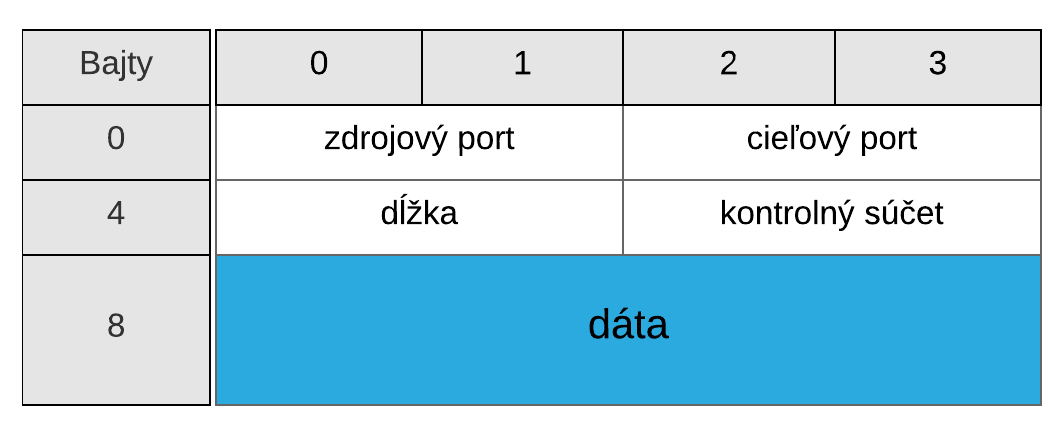
\includegraphics[width=.80\textwidth]{images/net-udp-head.png}
  \caption{Schéma popisujúca štruktúru UDP hlavičky a informácií}
  \label{fig:net-udp-head}
\end{figure}

\section{Sieťová vrstva}
Sieťová vrstva je skupina internetových definícií, protokolov a špecifikácií, ktorá
v sieťovom modeli TCP/IP slúži (transportnej vrstve) na prenos datagramov
(paketov) od odosielateľa, cez jednotlivé sieťové rozhrania, až k príjemcovi.
Každý z uzlov v sieti je na sieťovej vrstve identifikovaný takzvanou IP
\textit{(Internte Protocol)} adresou. Táto vrstva teda odvodzuje svoj názov od
svojej hlavnej funkcionality, ktorou je formovanie a tvorba pripojenia k
internetovej sieti prostredníctvom navzájom prepojených uzlov.

Protokoly sieťovej vrstvy pracujú s paketmi založenými na IP adresách
jednotlivých zariadení. Jednoznačne najznámejším protokolom tejto vrstvy je už
spomínaný IP \textit{(Internte Protocol)}. Sieťová vrstva však definuje aj iné
dôležité protokoly ako napríklad: ICMP
\textit{(Internet Control Message Protocol)}, ktorý slúži na odosielanie
chybových správ operačnými systémami, alebo IGMP
\textit{(Internet Group Management Protocol)} pre podporu multicastu smerovačov.
Neobsahuje však žiadne protokoly, ktoré definujú komunikáciu na
úrovni lokálnej podsiete a fyzických spojení.

\subsection{Protokol IP}
IP protokol sieťovej vrstvy je zodpovedný za adresáciu hostiteľského uzla a
prenos datagramu (paketu) od odosielateľa k príjemcovi cez jednu, alebo viacero
IP sietí. Pre tento účel definuje IP vlastný formát hlavičky paketov, čím
poskytuje logiku jednoznačnej identifikácie v rámci siete. Štruktúru hlavičky
IP paketu znázorňuje nasledujúci diagram.

\begin{figure}[h]
  \centering
    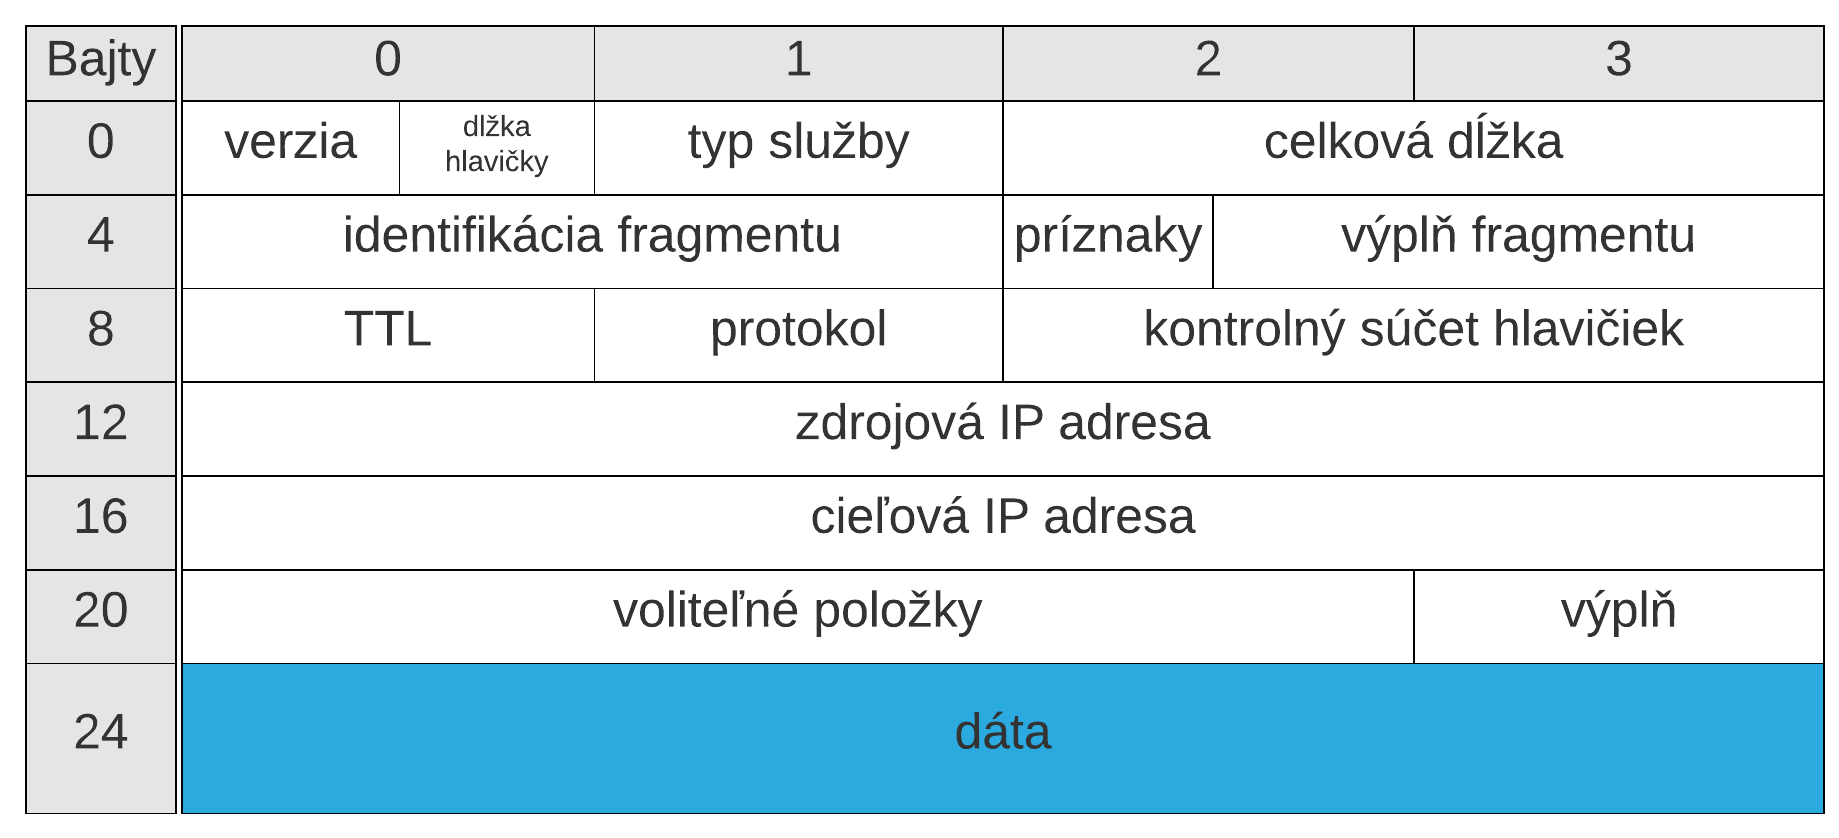
\includegraphics[width=.95\textwidth]{images/net-ip-head.png}
  \caption{Schéma popisujúca štruktúru hlavičky IP protokolu}
  \label{fig:net-ip-head}
\end{figure}

V skutočnosti existujú dve verzie IP protokolu: IP verzia 4 a IP verzia 6.
Každá z týchto verzií definuje štruktúru IP adries rozdielne. IP adresy v IPv4
sú 32 bitové, čo obmedzuje ich počet na približne 4,2 miliardy adries. Z tohto
počtu sú niektoré konkrétne adresy rezervované na špeciálne účely, ako napríklad
privátne siete (~18 miliónov adries), alebo adresy určené pre multicast
(~270 miliónov). Rapídny pokles počtu voľných IPv4 adries preto vyústil do
rozšírenia protokolu o IPv6. IPv6 definuje 128 bitové adresy, z čoho vyplýva,
že poskytne 3.4x1038 adries. Tento počet by mal byť do budúcna viac ako
dostačujúci.

Zrejme najzaujímavejšou informáciu z hľadiska identifikácie bude samotná IP
adresa, ktorá okrem identifikácie zariadenia poskytuje aj informáciu o
približnej polohe uzla, ktorému bola priradená. Podrobne sa problematike
identifikácie pomocou IP adries venuje kapitola \ref{ch:existing}. 

\section{Vrstva sieťového rozhrania}
Vrstva sieťového rozhrania pracuje v TCP/IP modeli na najnižšej úrovni.
Táto vrstva popisuje samotnú sieťovú architektúru a jej komunikáciu na úrovni
fyzického pripojenia. Ide o skupinu metód a komunikačných protokolov, ktoré 
teda operujú na fyzickom spojení dvoch uzlov.

Niektorými z jej dôležitých protokolov sú: ARP
\textit{(Address Resolution Protocol)}, RARP
\textit{(Reverse Address Resolution Protocol)},
NDP \textit{(Neighbor Discovery Protocol)}, OSPF
\textit{(Open Shortest Path First)} a iné.

Informácie týchto protokolov však operujú na príliš nízkej úrovni sieťovej
infraštruktúry, preto ich nebude možné využiť pri identifikácii. V prehľade je 
teda vrstva sieťového rozhrania uvedená len pre úplnosť.

\chapter{Útoky typu \textit{Denial of Service}}
\label{ch:dos}
Jedným z hlavných dôvodov a motivácií identifikácie užívateľov je prevencia
proti útokom. Medzi najznámejšie z útokov, proti ktorým je možné brániť sa
práve týmto spôsobom, patrí takzvaný útok typu \textit{Denial of Service}
(ďalej len \textit{DoS}).

Vo všeobecnosti je za \textit{DoS} útok považovaná snaha útočníka zabrániť
oprávneným užívateľom v prístupe k informáciám, prípadne službám poskytovateľa.
Snahou útočníka je znefunkčniť pripojenie neustálym narúšaním služby serveru,
prípadne sieťovej infraštruktúry, v dôsledku čoho môže dôjsť k čiastočnej, či
úplnej strate pripojenia hostiteľa. 

\begin{figure}[h]
  \centering
    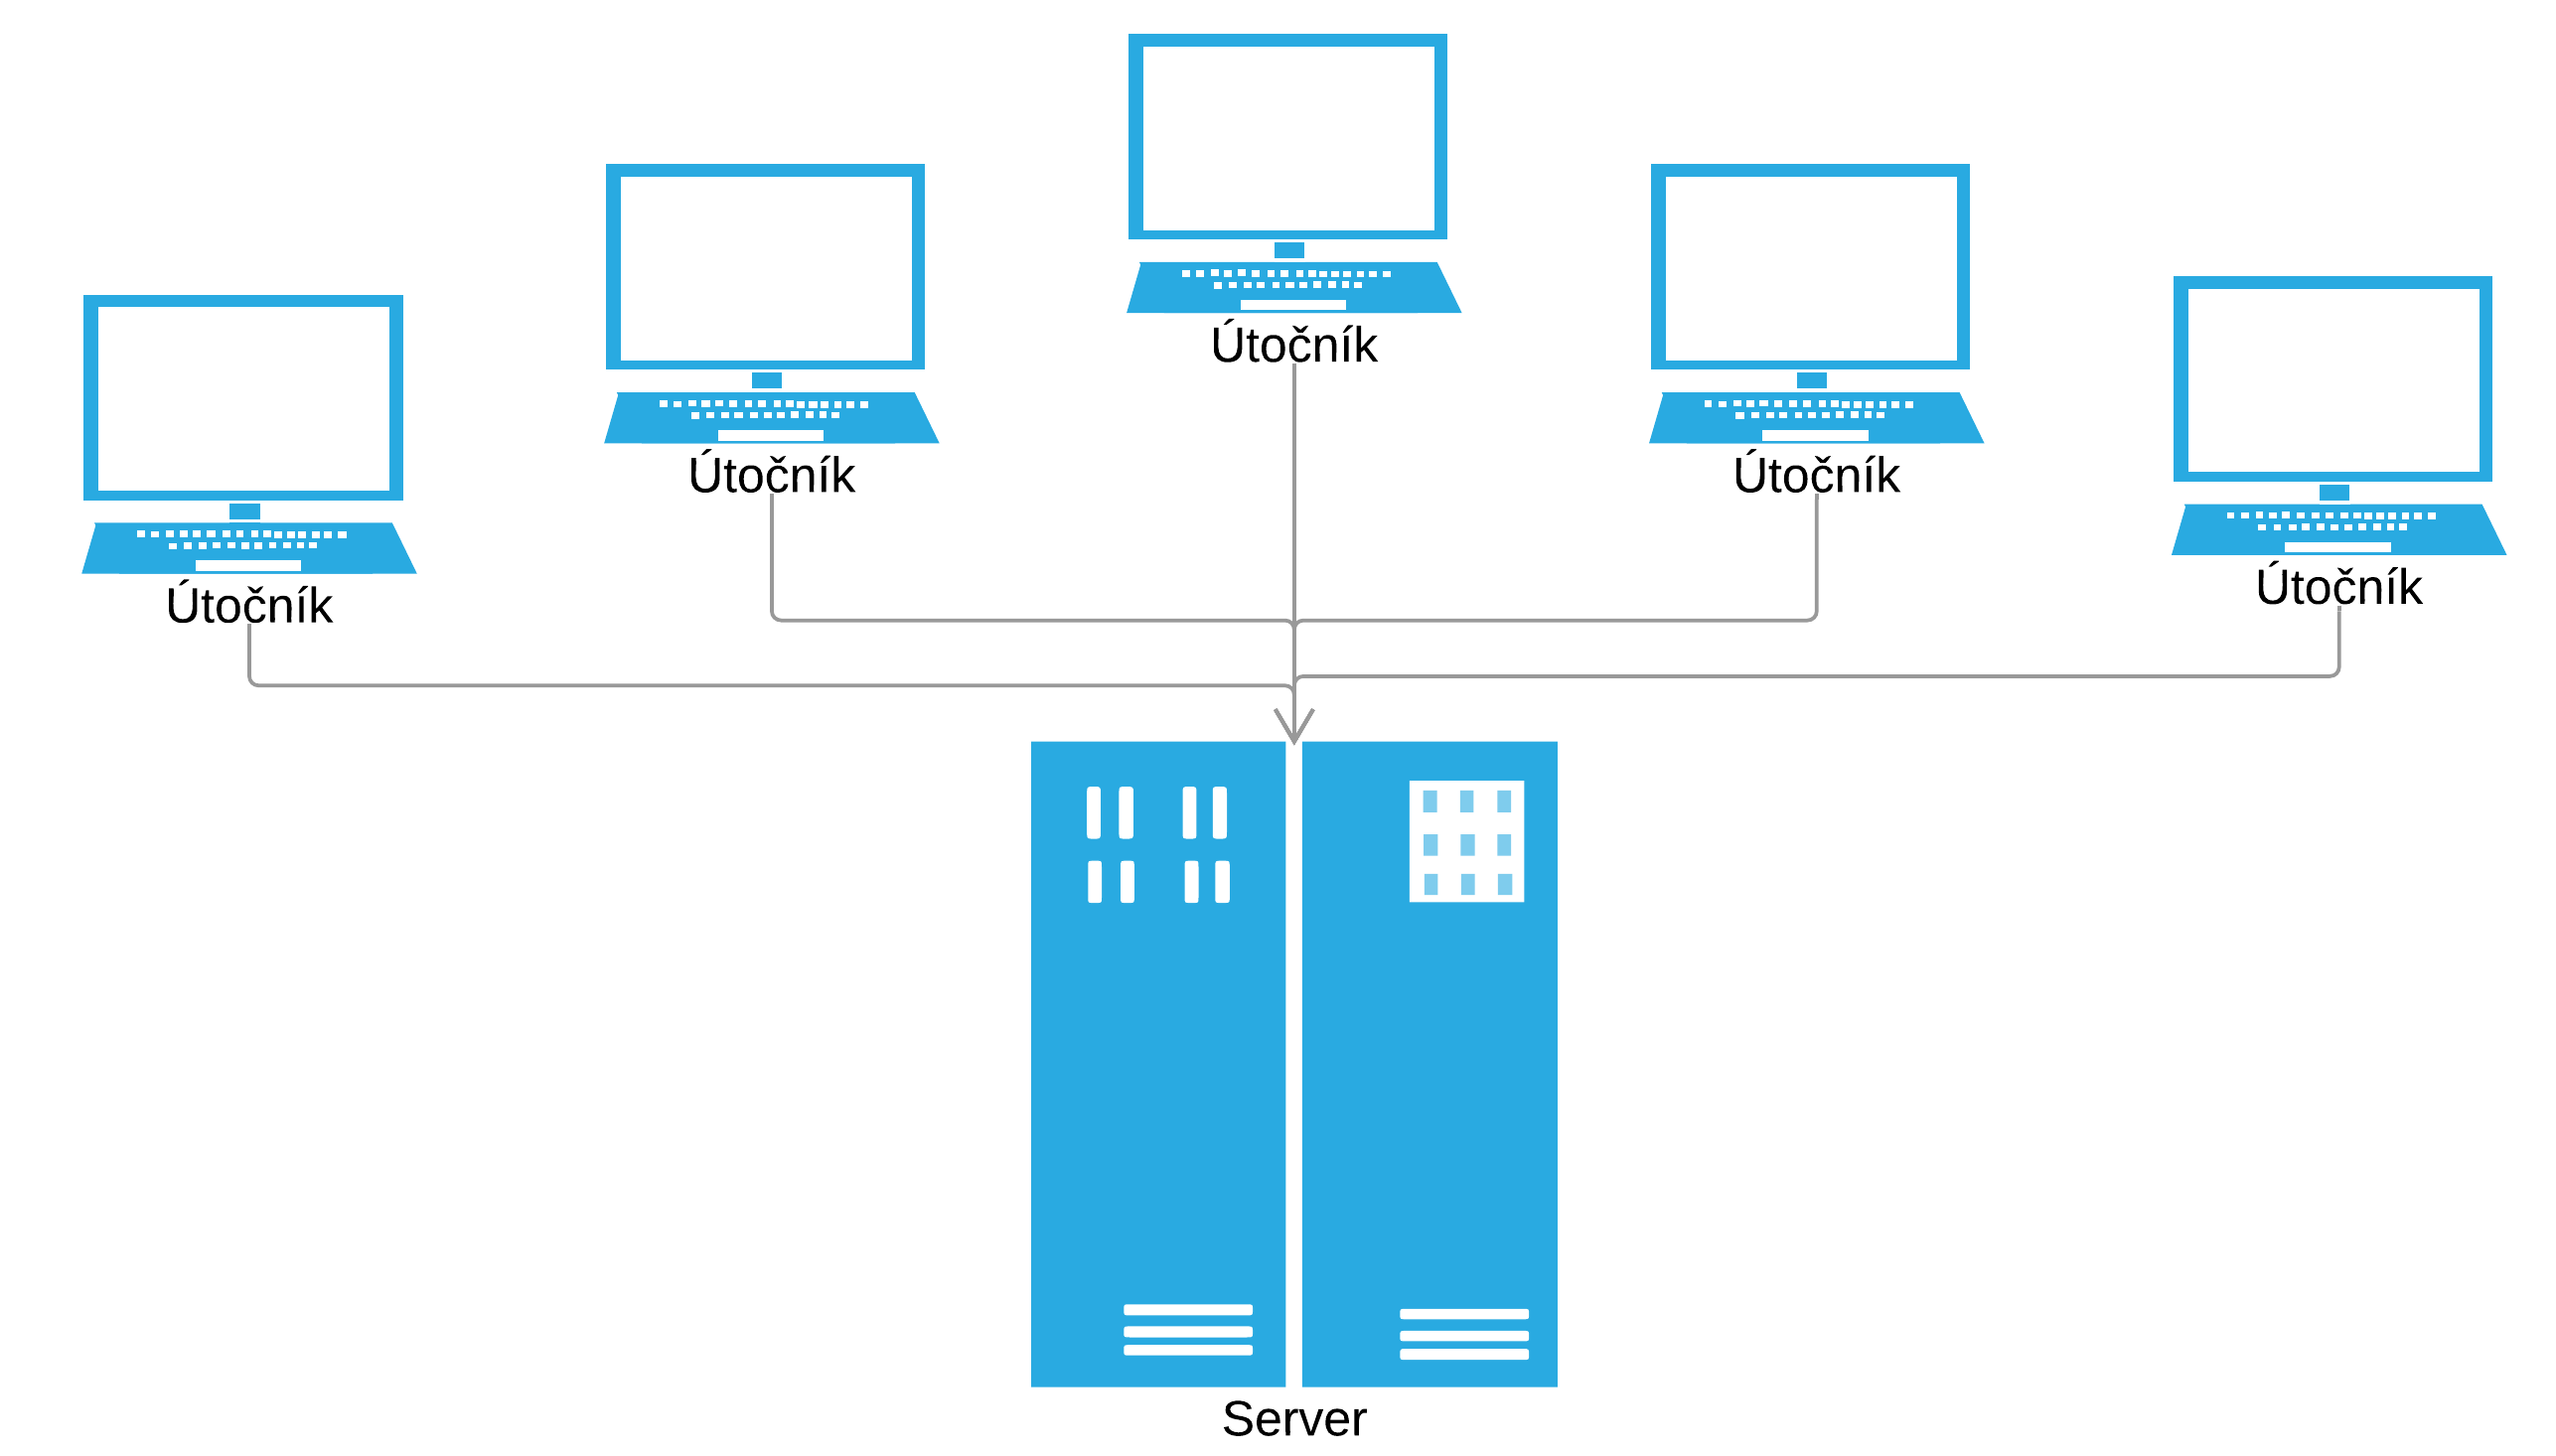
\includegraphics[width=\textwidth]{images/dos.png}
  \caption{Schéma DoS útoku, zdroj: vlastné spracovanie}
  \label{fig:dos}
\end{figure}

\section{Základne typy a techniky}
Existuje mnoho rôznych typov a techník vykonávania \textit{DoS} útokov.
Nasledujúce odseky preto popisujú najpoužívanejšie z nich a identifikujú
prostriedky, pomocou ktorých je možné sa im brániť.

\subsection{Distribuované DoS útoky}
O distribuovaných \textit{DoS} útokoch hovoríme v prípade, že viaceré zariadenia zaplavia
celú šírku pásma, prípadne zdrojov cieľového systému, ktorým je zvyčajne jeden, alebo viacero
serverov. Takýto útok je často dôsledkom použitia rôznych systémov a zariadení (napríklad
takzvaného \textit{botnetu}), ktoré sa snažia vyťažiť cieľový systém. \textit{Botnet} je rozsiahla
virtuálna sieť umelých (\textit{zombie}) počítačov, ktorých cieľom je prijímať príkazy bez
vedomia majiteľa. Keď cieľový systém spotrebuje všetky voľné spojenia, ďalšie už nie
je možné nadviazať. 

\begin{figure}[h]
  \centering
    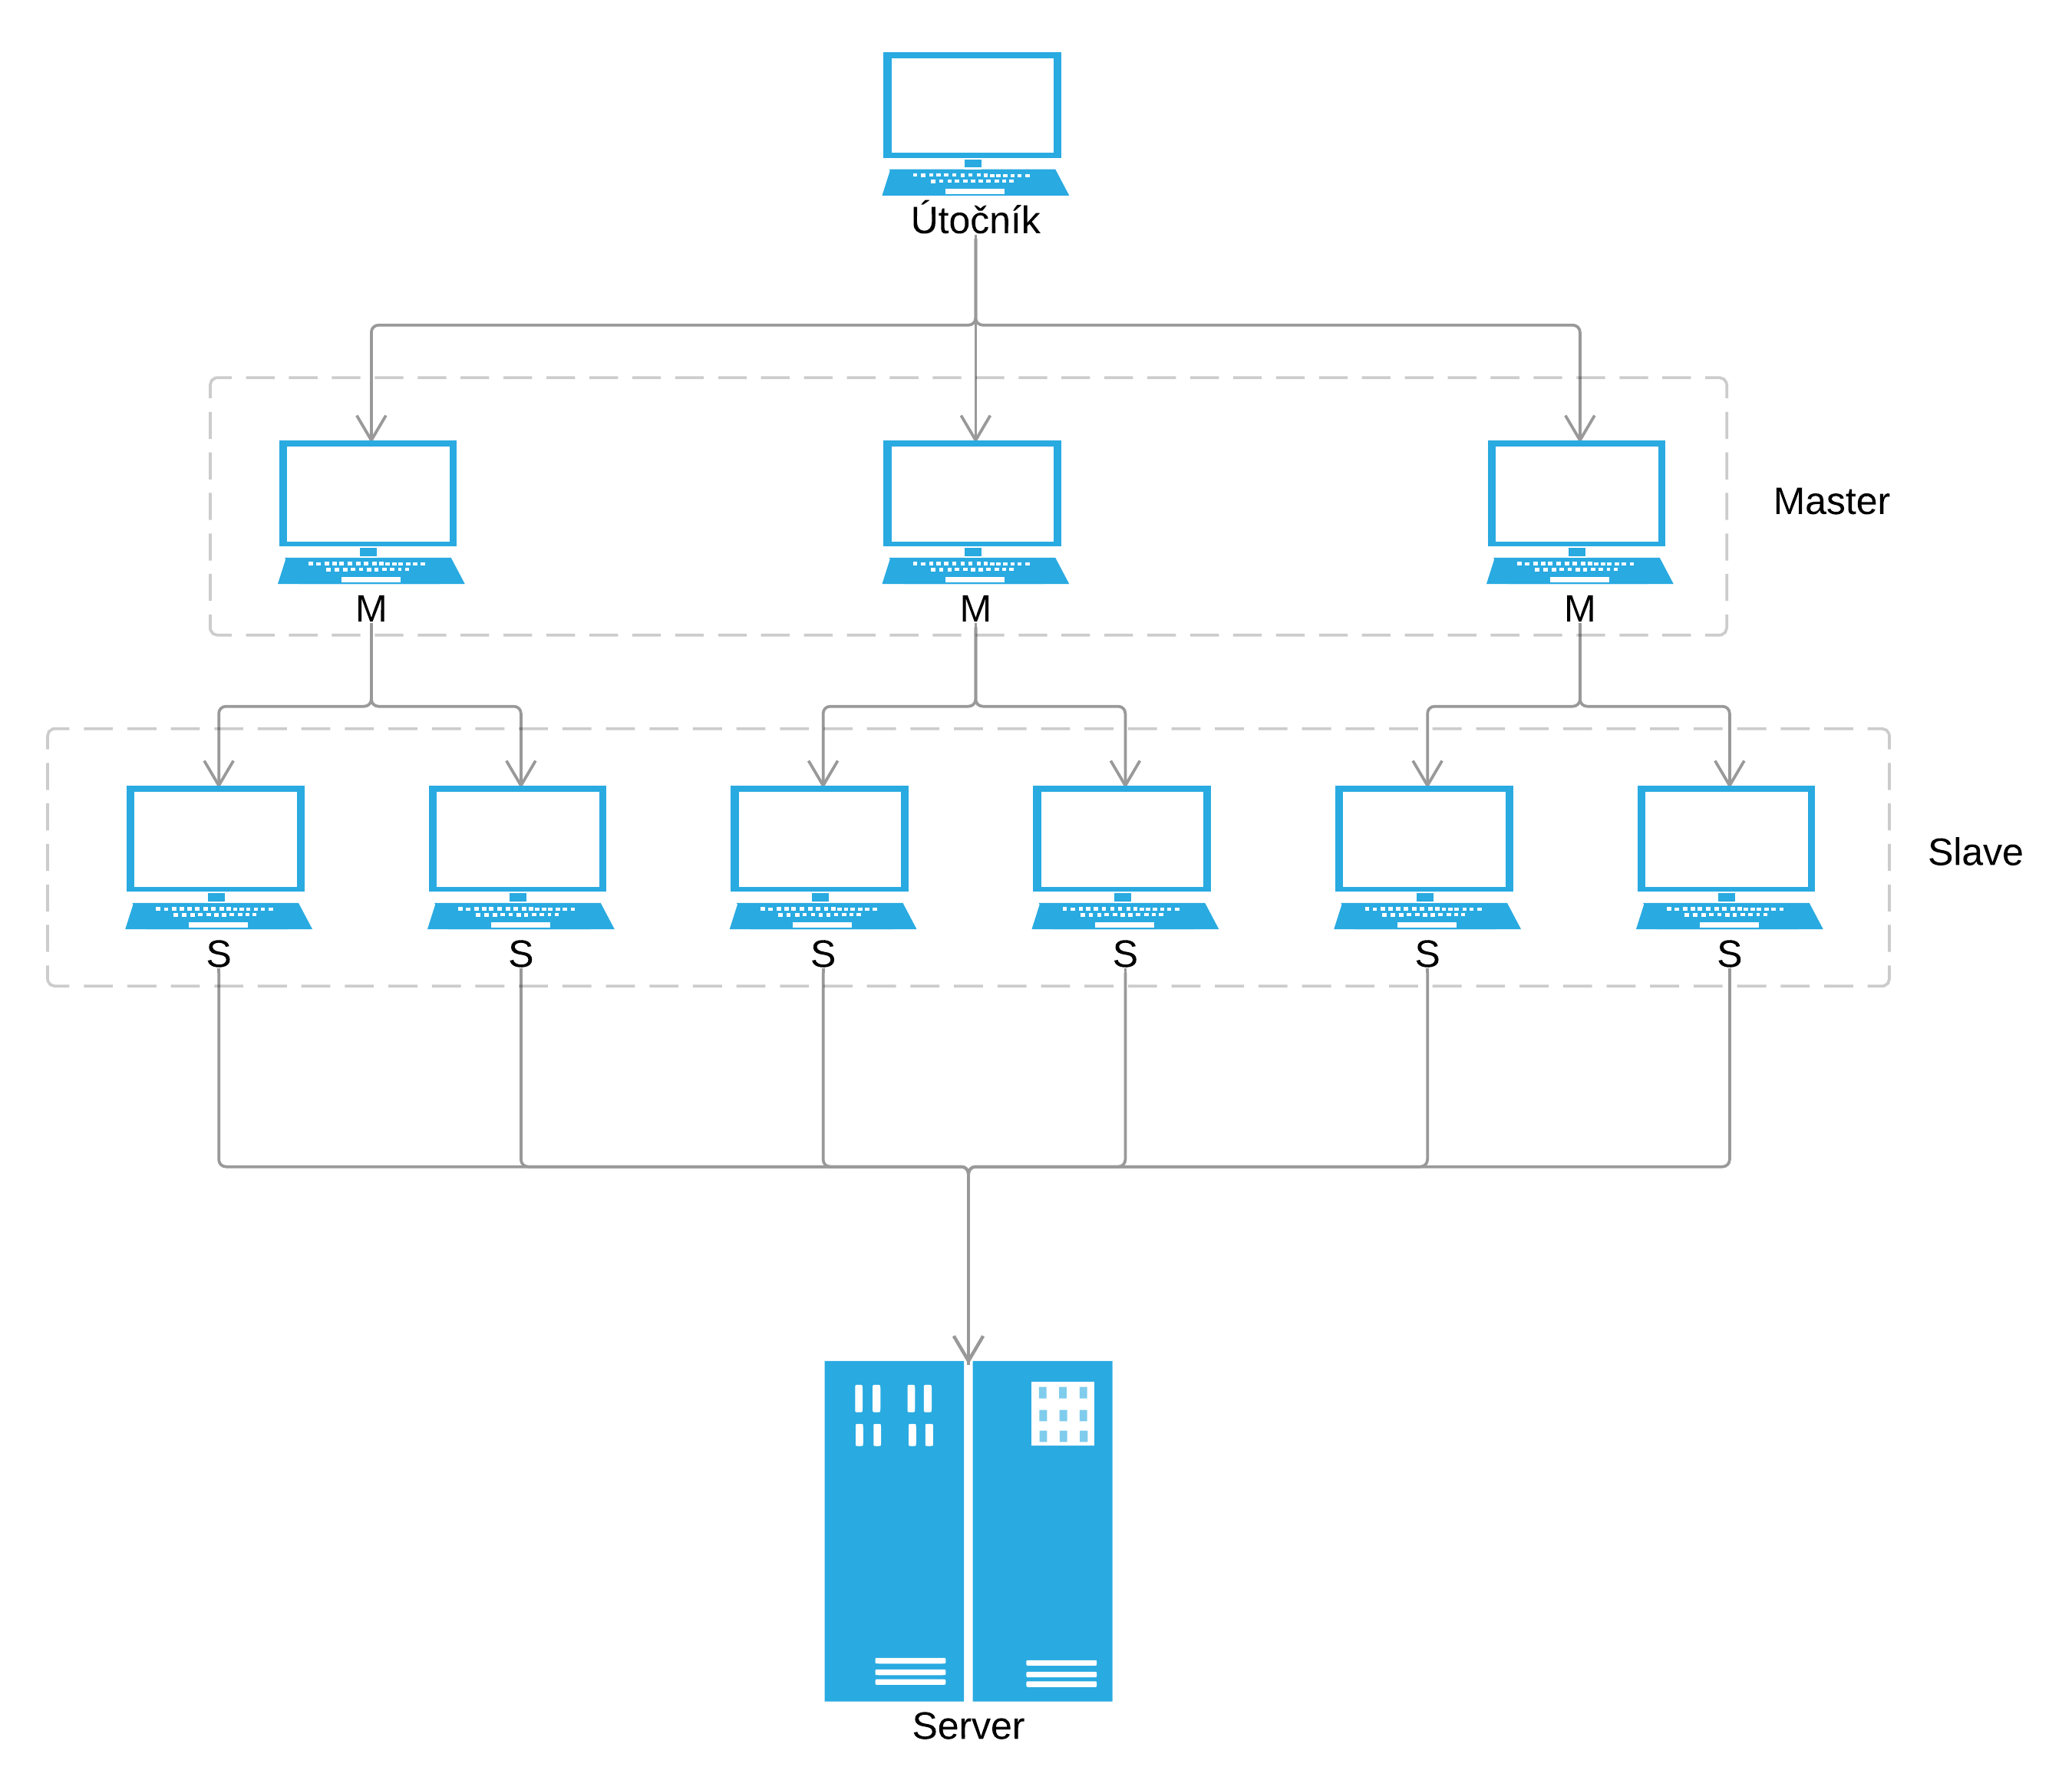
\includegraphics[width=\textwidth]{images/ddos.png}
  \caption{Schéma rozloženia DDoS útoku, zdroj: vlastné spracovanie}
  \label{fig:ddos}
\end{figure}

Hlavné výhody útočníka pri využití Distribuovaného \textit{DoS} útoku
spočívajú v skutočnostiach, že viaceré zariadenia dokážu generovať väčšiu záťaž ako jedno,
pričom použitie množstva systémov zabezpečuje omnoho ťažšiu detekciu jeho identity. Správanie
sa každého z týchto zariadení je zároveň horšie pozorovateľné, čo sťažuje obranu voči samotnému útoku.

Tieto výhody taktiež spôsobujú vývoj obranných mechanizmov. Na strane cieľového serveru už
nebude stačiť jednoduché zvýšenie šírky pásma nad hranicu momentálnej veľkosti útoku, pretože
útočník môže napríklad zvýšiť počet zapojených zariadení, čím by taktiež spôsobil zaťaženie a
výpadok systému.

\subsection{Sémantické DoS útoky}
Sémantické útoky využívajú špecifickú funkcionalitu alebo implementačnú chybu aplikácie,
prípadne protokolu zariadenia obete na zneužitie určitého množstva jeho zdrojov. Napríklad
v prípade \textit{TCP SYN} útoku je touto zneužitou funkcionalitou alokácia značného množstva
priestoru čakajúcich pripojení ihneď po potvrdení \textit{ TCP SYN requestu}. Útočník otvorí
viaceré spojenia, ktoré nikdy neuzavrie, čím zahlcuje server. 

Pri \textit{CGI} útoku je zasa cieľom útočníka takýmto spôsobom zahltiť procesor viacerými
\textit{CGI requestami}.

Jedným z obzvlášť nebezpečných útokov je \textit{NAPTHA} útok, ktorý sa zameriava na
\textit{TCP} protokol. Inicializuje mnoho \textit{TCP} spojení, ktoré zaplnia zdroje serveru.

\subsection{Reflexia a amplifikácia}
U reflexie (\textit{DRDoS}) je za reflektujúce zariadenie považovaná akákoľvek hostiteľská IP adresa, 
ktorá v prípade odoslania
paketu, tento paket spätne aj vráti.
Skupiny útočníkov cielene organizujú nimi kontrolované hostiteľské servery tak, aby sa zasielali 
falošné dáta, simulujúce napadnutý uzol, až ku reflektujúcemu serveru. Vo výsledku sú teda obete 
napadnuté z výrazne väčšieho počtu zdrojových bodov, obsiahlo rozptýlených v sieti, čím útočníci účelne 
odrezávajú ich spojenie zo zvyškom Internetu.

Amplifikačný útok je typ reflektujúceho útoku, kde reflektujúci server odosiela mnohonásobne väčší 
objem odpovedí, než prijíma. Týmto spôsobom teda znásobuje aj vyťaženie spojenia medzi obeťou a 
zdrojovým uzlom.

\begin{figure}[h]
  \centering
    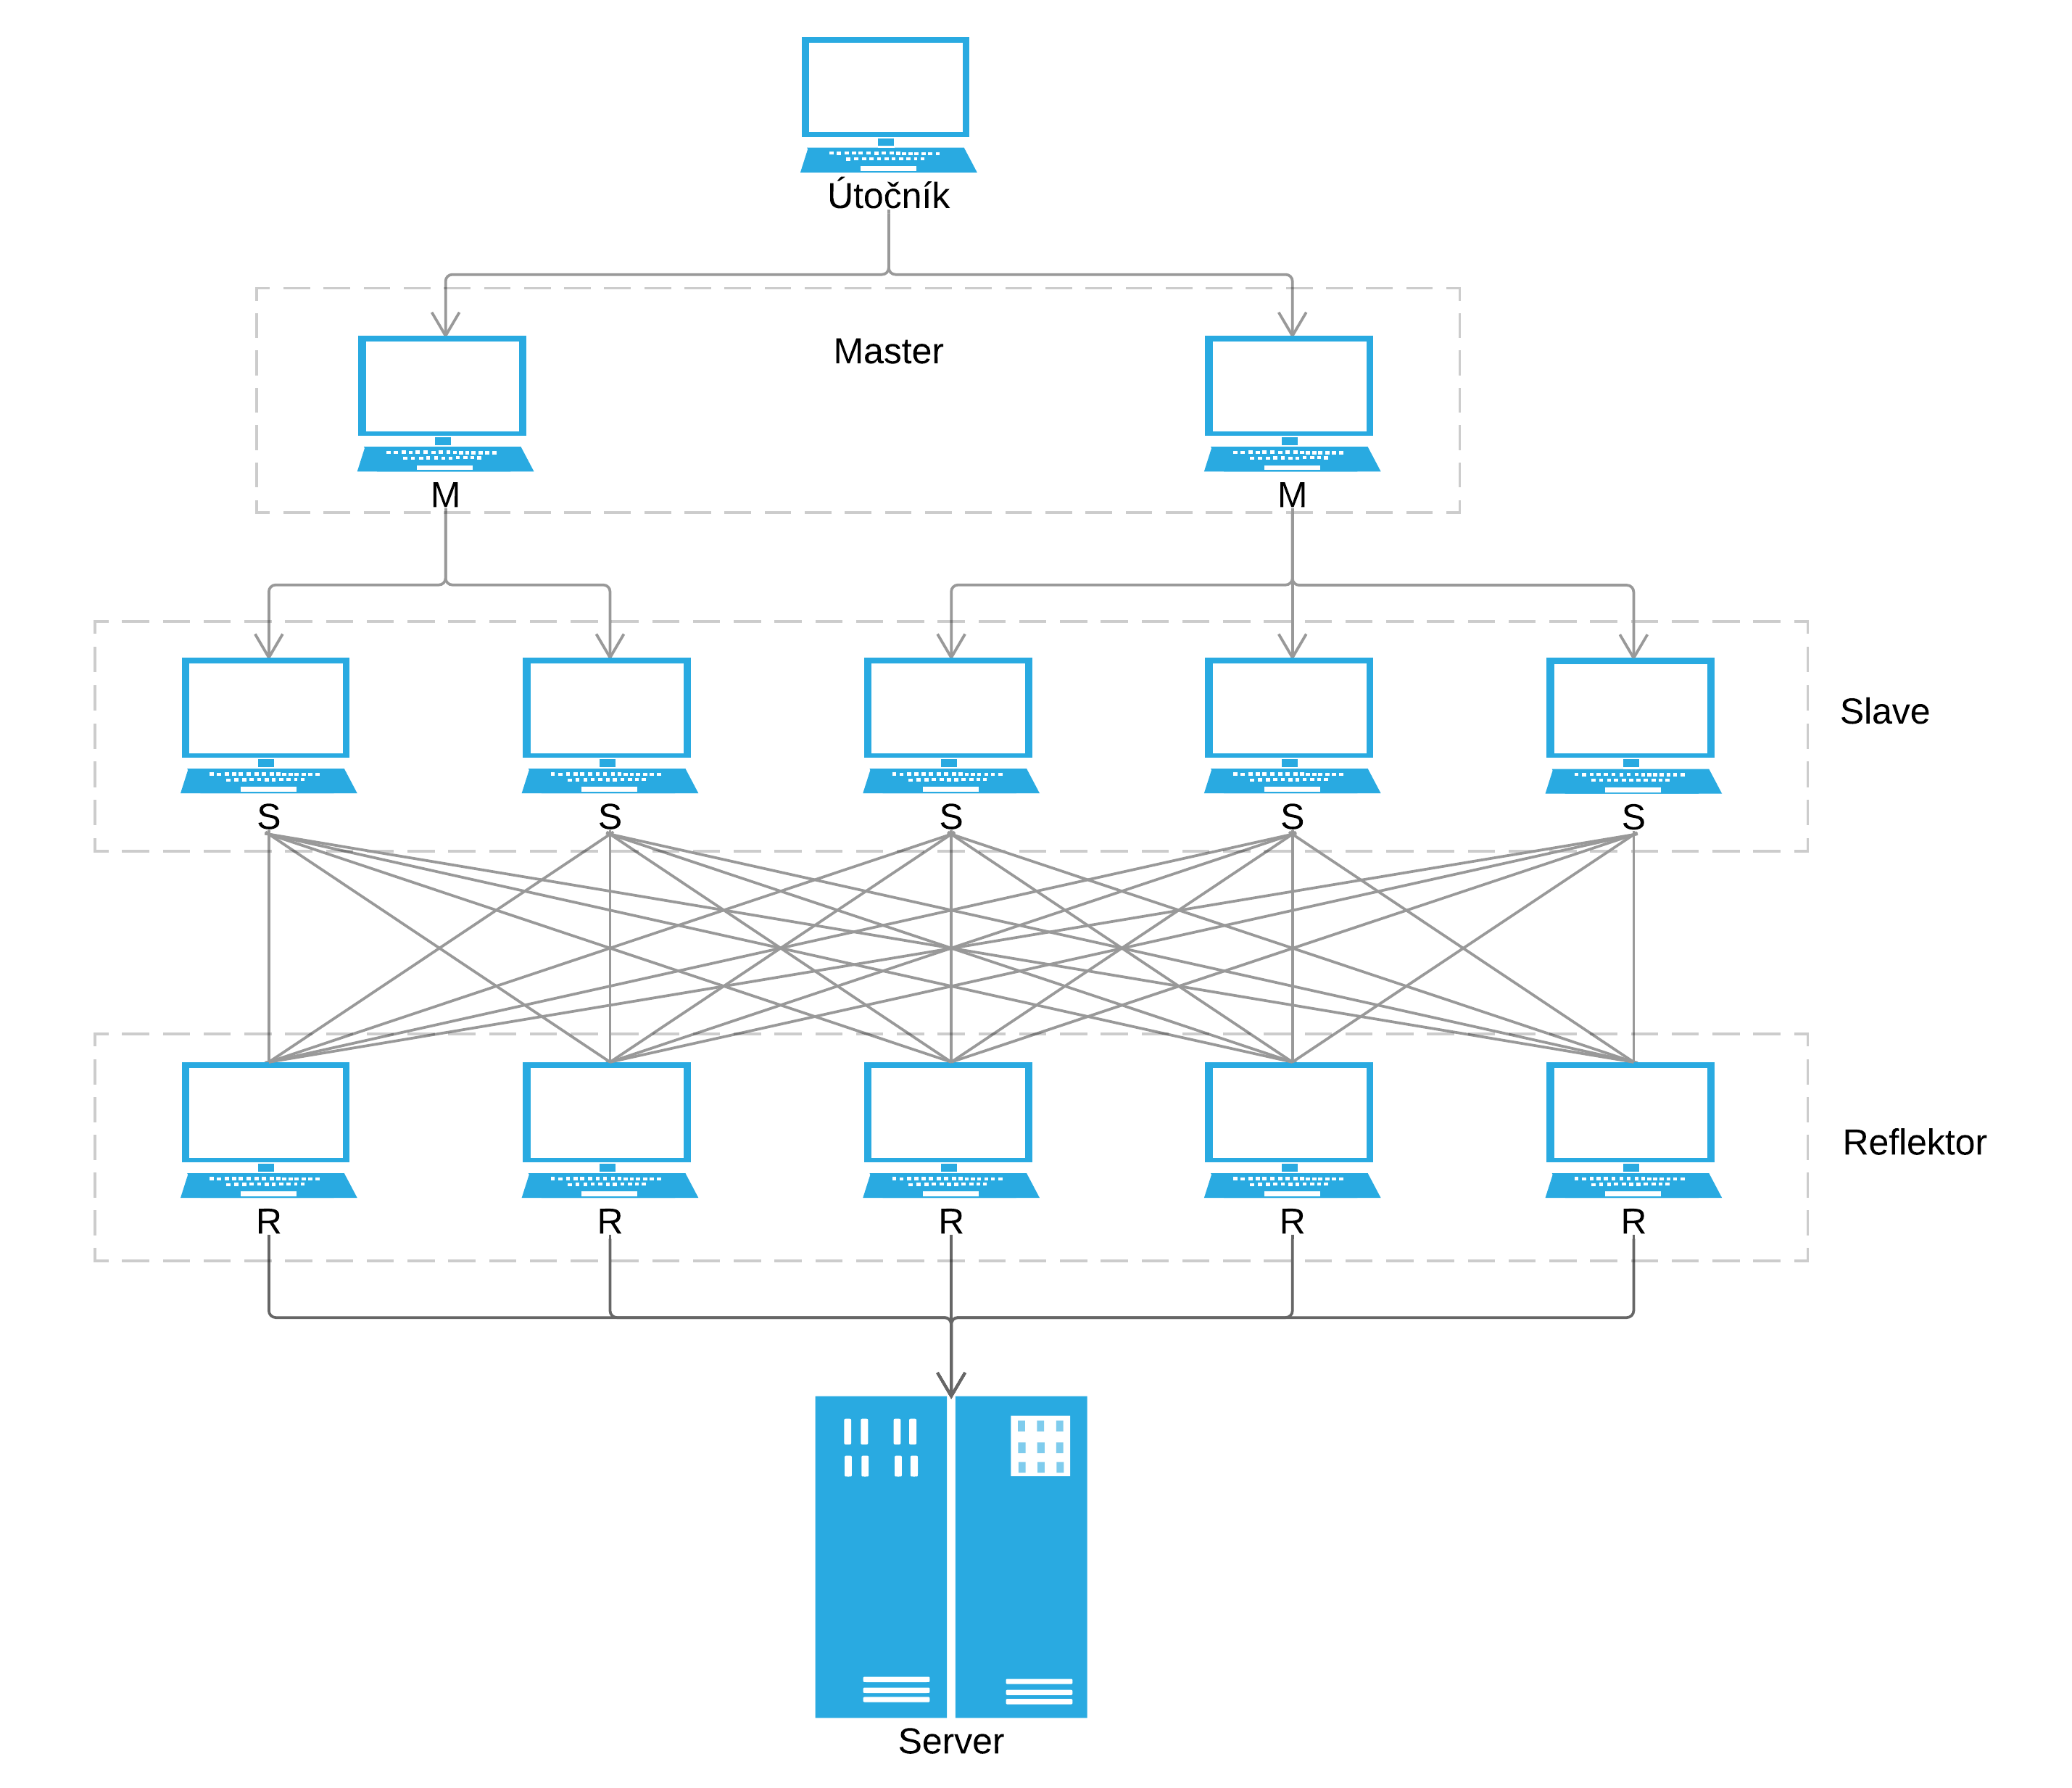
\includegraphics[width=\textwidth]{images/drdos.png}
  \caption{Schéma rozloženia DRDoS útoku, zdroj: vlastné spracovanie}
  \label{fig:drdos}
\end{figure}

%\subsection{HTTP POST DoS útoky}
%Výskyt kompletného HTTP POST útoku s legitímnou hlavičkou, v ktorej je obsiahnutá ’Content-Length’ položka,  špecifikujúca veľkosť tela sprievodnej správy, sa prvý raz objavil v roku 2009. Útočník však realizuje zaslanie skutočného tela správy extrémne pomalou rýchlosťou, ako napríklad 1 byte za 110 sekúnd. So zámerom uchovať celú správu korektnú a kompletnú, cieľový server sa bude pokúšať riadiť podľa ’Content-Length’ pola v hlavičke a čakať, kým nie je celé telo správy prenesené, čo može trvať skutočne dlho. Útočník zriadi stovky, či dokonca tisíce takýchto pripojení, pričom sú všetky vstupné body prichádzajúcich pripojení (obetí)  využité na znemožnenie vytvárania ďaľších (včetne legitímnych) pripojení, pokým sa neodošlú všetky dáta.

% First discovered in 2009, the HTTP POST attack sends a complete, legitimate HTTP POST header, which includes a 'Content-Length' field to specify the size of the message body to follow. However, the attacker then proceeds to send the actual message body at an extremely slow rate (e.g. 1 byte/110 seconds). Due to the entire message being correct and complete, the target server will attempt to obey the 'Content-Length' field in the header, and wait for the entire body of the message to be transmitted, which can take a very long time. The attacker establishes hundreds or even thousands of such connections, until all resources for incoming connections on the server (the victim) are used up, hence making any further (including legitimate) connections impossible until all data has been sent. 

%Je pozoruhodné, že na rozdiel od množstva iných (D)DoS útokov, ktoré sa pokúšali pokoriť server preťažením svojej siete alebo CPU, HTTP POST útok je zameraný na logické možnosti svojich obetí.V praxi to znamená, že zasiahnutým prvkom ostane dostatok network bandwidth priepustnosti vrámci siete a výkonu procesoru na nenarušenú prevádzku. V neposlednom rade, ak zvážime, že softvérový webový server Apache implicitne akceptuje požiadavky o veľkosti 2 GB, môže byť tento typ útoku obzvlášť silný. Je veľmi ťažké ich odlíšiť od neškodných legitímnych pripojení, preto sú schopné obísť aj bezpečnostné systémy. 
%OWASP (open source web application security project) poskytla verejnosti testovací prostriedok pre overovanie bezpečnosti serverov voči takémuto druhu nástrahy.

%It is notable that unlike many other (D)DoS attacks, which try to subdue the server by overloading its network or CPU, a HTTP POST attack targets the logical resources of the victim, which means the victim would still have enough network bandwidth and processing power to operate. Further combined with the fact that Apache will, by default, accept requests up to 2GB in size, this attack can be particularly powerful. HTTP POST attacks are difficult to differentiate from legitimate connections, and are therefore able to bypass some protection systems. OWASP, an open source web application security project, has released a testing tool to test the security of servers against this type of attacks.

\section{DoS nástroje a DoS as a Service}
Typickou metódou prenosu mechanizmov \textit{DoS} a \textit{DDoS} útokov je malvér. Jedným z príkladov 
bol
takzvaný \textit{MyDoom}. Ide o \textit{DoS} mechanizmus, ktorý sa spúšťal vo vopred naplánovanom čase.
Tento útok zahŕňal nastavenie hodnoty \textit{IP} adresy cieľového systému pre nasadenie malvéru,
pričom pre spustenie útoku nebola potrebná žiadna interakcia s používateľom.

Ďalším spôsobom zneužitia systému pre \textit{DDoS} útok je použitie skrytej časti softvéru tretej
strany, ktorý umožní útočníkovi stiahnutie \textit{zombie} agenta, prípadne ho už softvér sám obsahuje.
Útočník môže preniknúť do systému taktiež pomocou automatizovaných nástrojov, ktoré zneužívajú chyby v
programoch počúvajúcich vzdialené pripojenia. Tento scenár zasahuje primárne systémy, ktoré sa správajú
ako webové servery. Typickým príkladom \textit{DDoS} nástroja z tejto oblasti je takzvaný
\textit{Stacheldraht}. \textit{Stacheldraht} využíva vrstevnatú štruktúru, v ktorej útočník používa
program klienta na pripojenie sa k \textit{handlerom}, ktoré sú zneužívané na prenos príkazov
k \textit{zombie} agentom. Agenti následne vykonávajú samotný \textit{DDoS} útok. Agenti sú cez 
handleri
zneužívaní útočníkom za pomoci použitia automatizovaných algoritmov na vyhľadávanie zraniteľností v
programoch, ktoré prijímajú vzdialené pripojenia. Každý \textit{handler} je schopný kontrolovať až 
tisíc
agentov. 

DDoS nástroje ako \textit{Stacheldraht} stále používajú klasické \textit{DoS} metódy zamerané na
zosilnenie a podvrhovanie IP adries, ako napríklad útok vyťaženia šírky pásma. Ďalšou z možností je
zahltenie zdrojov - \textit{SYN Flood} útok. Novšie nástroje používajú na \textit{DoS} útoky taktiež
\textit{DNS} servery.

Nástroje ako \textit{MyDoom} môžu byť použité voči ľubovoľnej IP adrese. Menej skúsení útočníci ich
používajú k znemožneniu dostupnosti populárnych a známych webových serverov. Naopak sofistikovanejší
útočníci používajú tieto nástroje na vydieranie, napríklad voči svojim obchodným protivníkom.

V niektorých prípadoch sa však môže zariadenie stať časťou \textit{DDoS} útoku zámerne - so súhlasom
majiteľa. Príkladom je distribuovaný útok \textit{Operation Payback} organizovaný skupinou
\textit{Anonymous}.

%---

%%TODO DoSaaS

%Typicky sa pre tieto účely používa LOIC. Spolu s HOIC je dnes k dispozícii široká škála nástrojov DDoS, vrátene platených, ale aj ich neplatených verzií, s rôznymi funkcionalitami.
%Všetko je dostupné vrámmci rozvinutého čierneho trhu - na fórach, ktoré sú s oblubou navštevované hekermi, alebo na rôznorodých IRC kanáloch.
%Britská GCHQ vyvinula nástroje pre  DDoS, pomenované PREDATORS FACE a ROLLING THUNDER.
%Niektorí predajcovia poskytujú takzvané "booterör "stresser" služby, ktoré majú jednoduché webové rozhranie, prostredníctvom ktorého umožňujú akceptovať platby cez web. Tieto trhom nesmierne propagované nástoje možu byť zneužité na vykonanie neautorizovaného útoku, pod maskou odmietnutia služby. Poskytnú tak útočníkovi technicky bezproblémový prístup pre sofitikovaný útok bez potreby najskôr porozumieť načo je príslušná služba využívaná.

% The LOIC has typically been used in this way. Along with HOIC a wide variety of DDoS tools are available today, including paid and free versions, with different features available. There is an underground market for these in hacker related forums and IRC channels.

% UK's GCHQ has tools built for DDoS, named PREDATORS FACE and ROLLING THUNDER.

% Some vendors provide so-called "booter" or "stresser" services, which have simple web-based front ends, and accept payment over the web. Marketed and promoted as stress-testing tools, they can be used to perform unauthorized denial-of-service attacks, and allow technically unsophisticated attackers access to sophisticated attack tools without the need for the attacker to understand their use.

\section{DoS - Zhrnutie}
Ako je možné vidieť z predchádzajúcich odsekov, existuje naozaj veľké množstvo
variácií \textit{DoS} a \textit{DDoS} útokov. Zároveň ich počet postupom času
narastá a preto je nutné vyvíjať nové nástroje na obranu voči nim. Najťažšou časťou
je však takýto útok, najmä jeho pôvodcu, odhaliť a identifikovať. Jedným z využití
algoritmu popísaného v kapitole \ref{ch:footprint} a implementačnej časti je preto
práve táto funkcionalita.

\chapter{Existujúce prístupy k identifikácií}
\label{ch:existing}
Dôležitou súčasťou tejto práce je popis existujúcich prístupov, ktoré
sú aktuálne využívané na účely identifikácie užívateľa. Práve ich porovnaniu
a hodnoteniu sa venuje nasledujúca kapitola.
Ide najmä o techniky využívajúce protokoly sieťovej vrstvy (najmä IP adresy),
monitorovanie TCP komunikácie a vlastné aplikačné identifikátory.

\section{Využitie sieťovej vrstvy}
Jedným z najtypickejších spôsobov identifikácie užívateľa a jeho zariadenia je
použitie informácií sieťovej vrstvy, predovšetkým jej IP protokolu.
Táto technika je veľmi rozšírená napríklad pre účely blokovania prístupu na
server, či u systémových \textit{firewallov}.

\subsection{Možnosti IP protokolu }
Ako popisuje kapitola \ref{ch:net-layers}, \textit{Internet Protocol} slúži na
prenos paketov medzi jednotlivými sieťovými uzlami - zariadeniami, ktoré sú
identifikované IP adresami. V ideálnom svete by bolo každé zariadenie v sieti
identifikované jednou statickou IP adresou. Bolo by teda možné užívateľa
rozpoznať len na základe množiny jeho adries. Bohužiaľ adresový priestor
protokolu IPv4 je obmedzený na 3.7 miliardy verejne dostupných adries
\footnote{
  Uvedené množstvo zahŕňa všetky možné dostupné IPv4 adresy - približne 4.2
  miliardy po odpočítaní rezervovaných adries - 588 miliónov.
}.
Z toho vyplýva potreba metód ich dynamického prideľovania, proxy serverov a
prekladu, čo identifikáciu značne komplikuje.

U dynamického prideľovania adries ide o jednoduché mapovanie pre zariadenia
na úrovni smerovača. Identifikácia je teda stále možná, len sťažená o vyšší
počet možných adries pre jedno zariadenie.

Preklad (\textit{Network Address Translation}) IP adries však identifikáciu
prakticky znemožňuje. Vo všeobecnosti ide o techniku prekladu jednej podmnožiny
IP adries na inú pomocou zmeny informácie o sieťovej adrese v datagrame IP
protokolu. Pôvodne sa táto technika používala pre zjednodušenie presmerovania
komunikácie bez nutnosti opätovnej adresácie každého uzla. 

V pokročilých
implementáciách však dnes \textit{NAT} predstavuje veľmi populárnu možnosť
takzvaného  IP maskovania. Maskovanie IP adries je technika zdieľania jednej
verejnej IP adresy celou privátnou podsieťou. Adresný priestor privátnej
podsiete, ktorá má byť skrytá je teda vždy mapovaný na verejnú IP adresu
smerovača. Táto adresa samotná je taktiež zvyčajne súčasťou väčšej podmnožiny
adresného priestoru. Pojem prekladu (\textit{NAT}) IP adries sa dnes už stal
synonymom ich maskovania. 

Paket odoslaný zo zariadenia, ktoré je prekryté
\textit{NAT} smerovačom bude teda ako zdrojovú adresu niesť namiesto IP adresy
zariadenia, z ktorého pochádza, hodnotu verejnej IP adresy smerovača.
Identifikácia na základe IP adresy preto v tomto prípade stráca význam.

\begin{figure}[H]
  \centering
    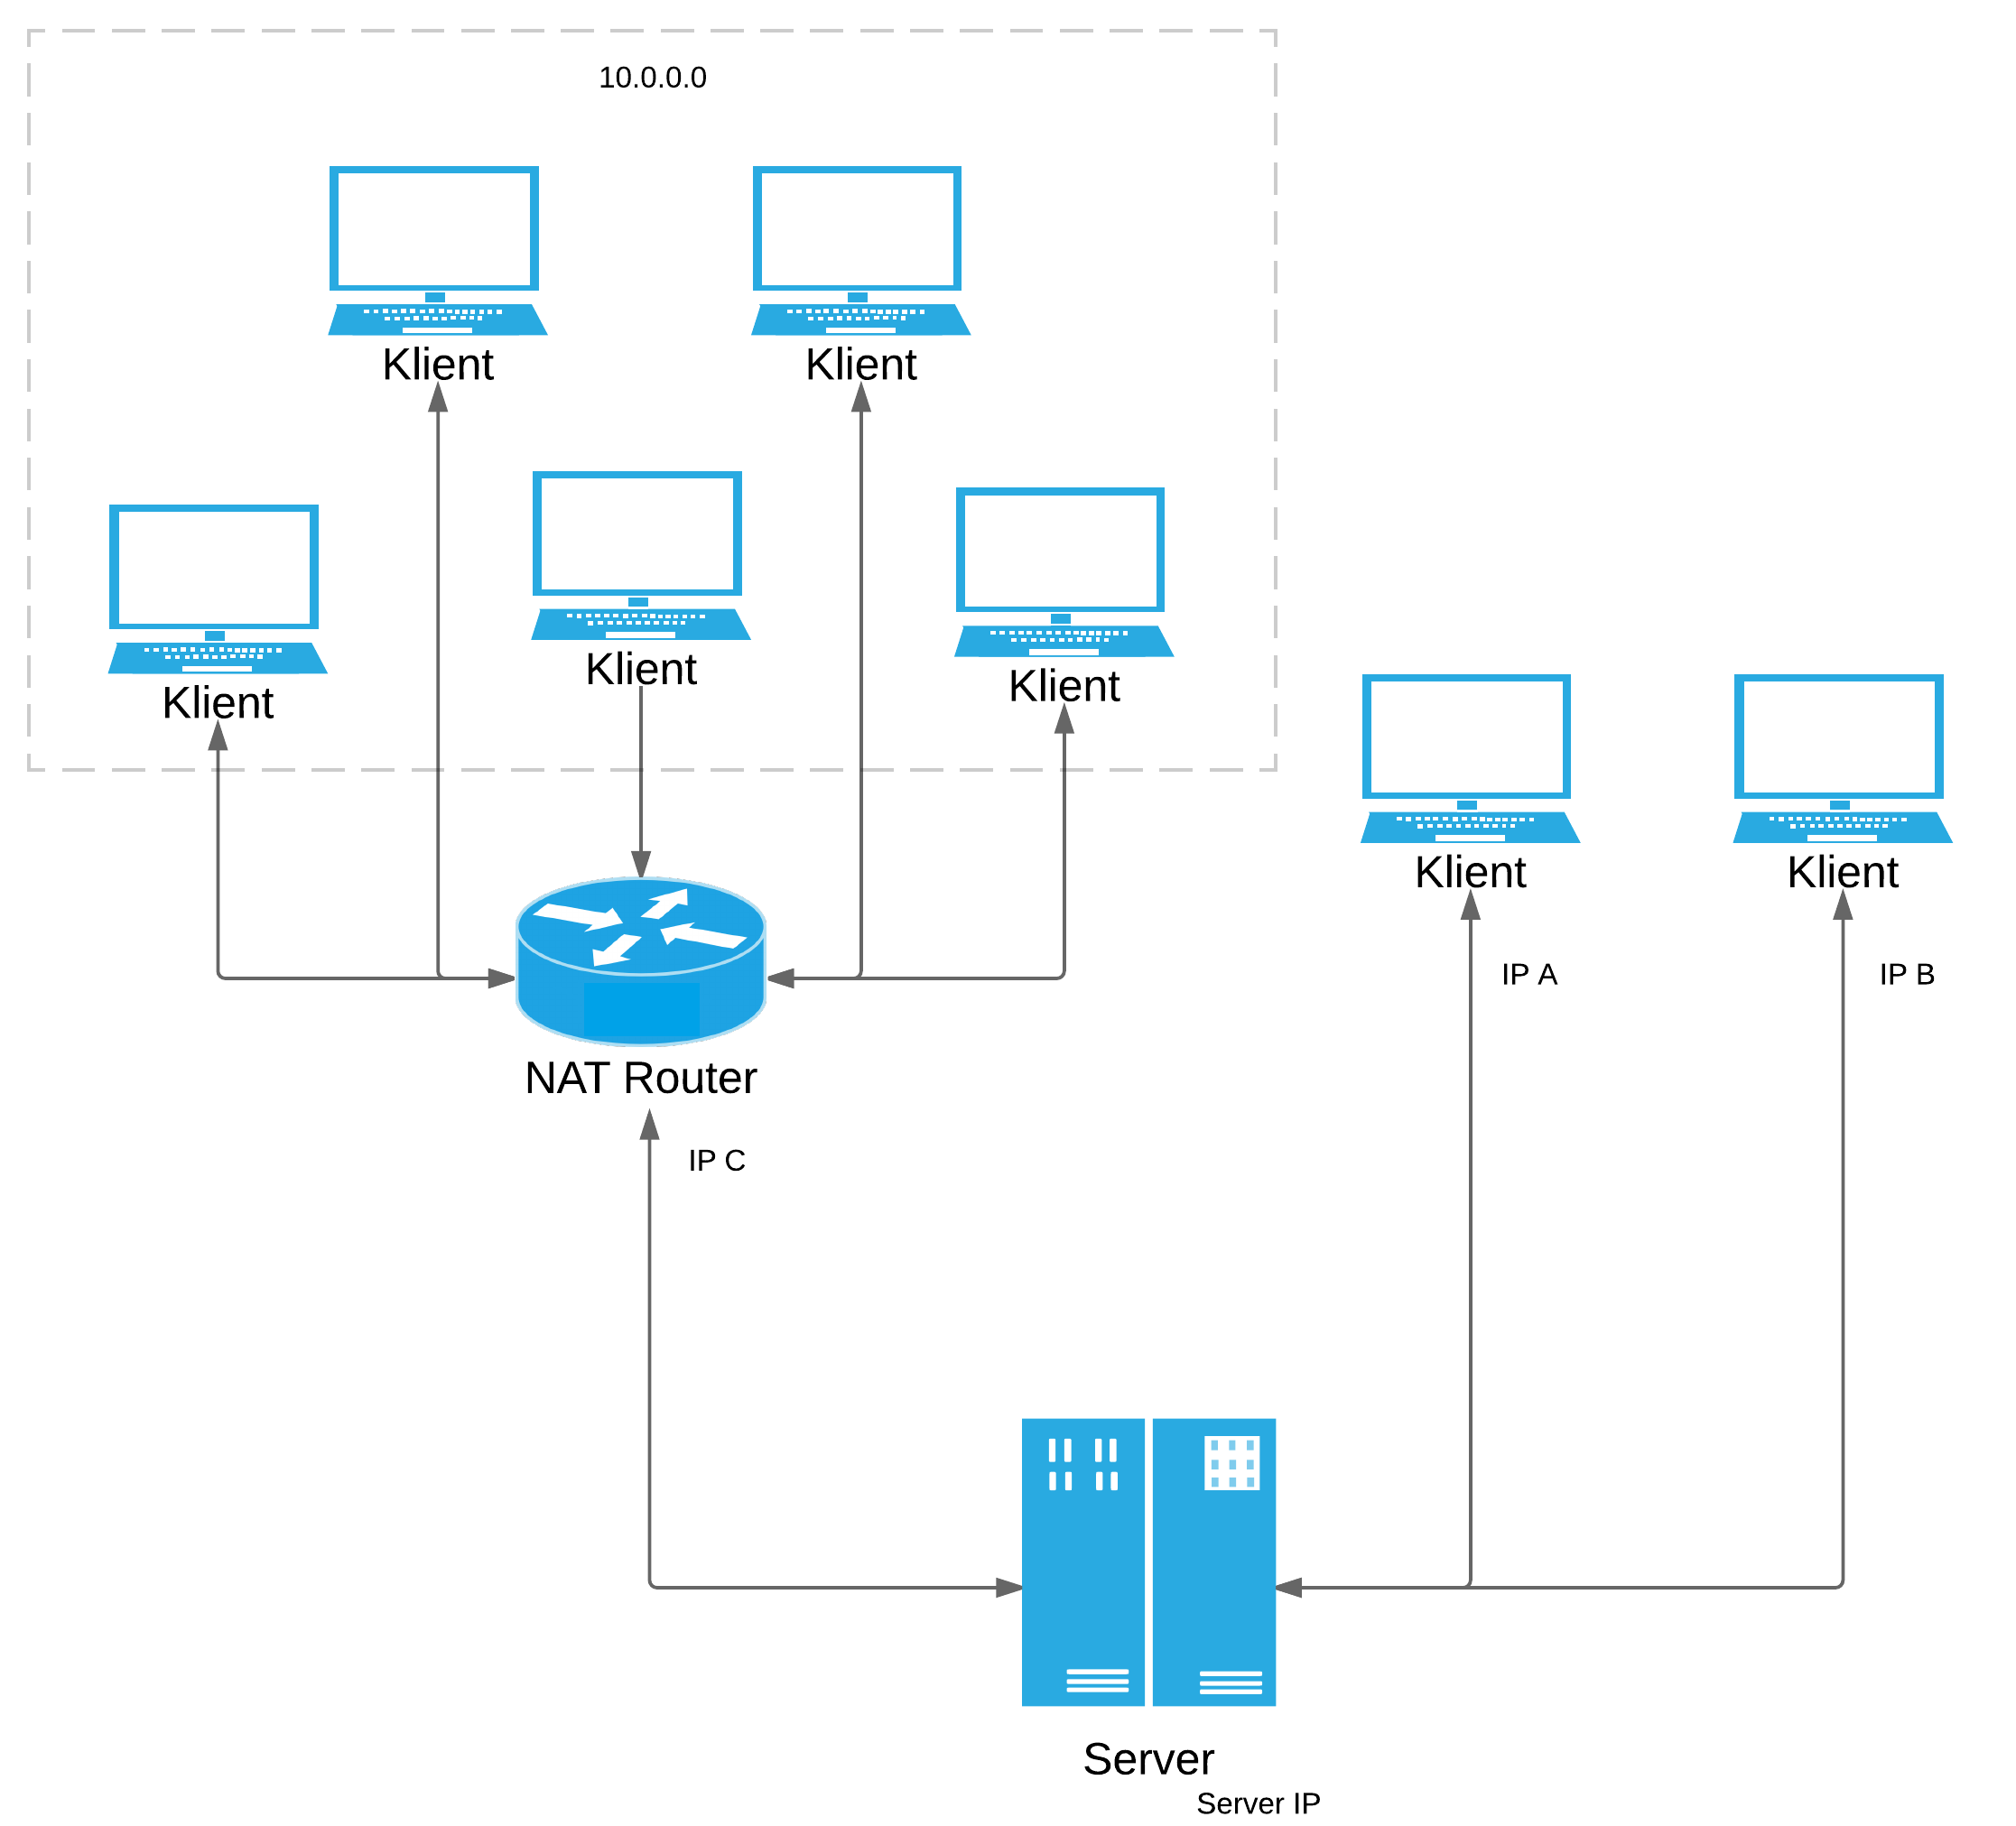
\includegraphics[width=.97\textwidth]{images/tech-IP-NAT.png}
  \caption{Vizualizácia rozloženia IP adresového priestoru pri použití techniky
  prekladu \textit{NAT}, zdroj: vlastné spracovanie}
  \label{fig:tech-IP-NAT}
\end{figure}

\subsection{Výhody a nevýhody IP}
Hlavnými výhodami použitia IP adries sú jednoduchosť, rýchlosť a flexibilita.
Napríklad pre účely znemožnenia prístupu stačí filtrovať len povolené IP
adresy, prípadne neumožniť prístup tým zakázaným. Oba spôsoby sú technicky veľmi
ľahko implementovateľné.

Ich nevýhodou je najmä rastúci trend použitia proxy serverov a \textit{NAT}
prekladu, čo má napríklad pri banovaní za následok znemožnenie prístupu aj
užívateľom, u ktorých to nie je potrebné, ale stoja za rovnakou IP adresou.

Vo všeobecnosti je teda identifikácia zariadení používateľa na základe IP
adresy možná. V prípade, že sa však zariadenie skrýva za proxy serverom,
prípadne sú adresy prekryté \textit{NATom} bude táto technika viesť takisto k
nechcenému prekrytiu jednotlivých užívateľov vrámci podsiete.

\section{Monitoring TCP}
Ako popisuje kapitola \ref{ch:net-layers}, TCP
\textit{(Transmission Control Protocol)} je jedným z protokolov transportnej
vrstvy sieťovej hierarchie, ktorého najtypickejším znakom je na rozdiel
od UDP garancia spoľahlivého doručenia paketov v presnom poradí. Prijatie
každého z paketov musí byť potvrdené príjemcom, inak je paket odoslaný znovu.
Poradie jednotlivých paketov je zaručené ich sekvenčnými číslami. Tieto 
vlastnosti robia z TCP jasnú voľbu pre aplikácie, ktoré vyžadujú nulovú
stratovosť dát. 

Aplikácie typicky zasielajú na TCP vrstvu \textit{stream} dát
pomocou takzvaných \textit{stream socketov}, čím sú dáta \textit{streamu}
rozdelené na primerane veľké segmenty. K segmentom je zároveň spočítaný
kontrolný súčet- \textit{TCP checksum}, pomocou ktorého je možné určiť, či
dáta neobsahujú poškodené pakety. Kontrolné súčty však nie sú v žiadnom ohľade
kryptograficky zabezpečené.\footnote{Podrobnému popisu štruktúry TCP paketu sa
taktiež venuje kapitola \ref{ch:net-layers}.}

Samotný TCP paket neobsahuje žiadne dáta, ktoré by mohli byť využité na priamu
identifikáciu používateľa (pokiaľ takéto informácie nie sú obsiahnuté v
nešifrovanej dátovej časti paketu), čo však neplatí pre IP protokol nižšej
úrovne. Zdrojové a cieľové porty TCP v spolupráci s IP adresou odosielateľa a
príjemcu môžu pomôcť identifikovať obe zúčastnené strany.

TCP je však dobrým príkladom doplnenia identifikácie na základe niekedy neúplných
informácií monitorovanej komunikácie. Táto neúplnosť spočíva napríklad v
spôsobe inicializácie položky sekvenčného čísla. Jej výpočet je definovaný,
počiatočná hodnota však zostáva neznáma. Možnosť výberu zostáva na vývojárovi,
pričom najčastejšie ide o náhodne zvolené číslo. To isté platí pre veľkosť TCP
okna (\textit{TCP Window}) používaného na ovládanie preťaženia. Nakoľko
riadenie preťaženia má kľúčový vplyv na celkový výkon TCP, veľa pokusov o
optimalizáciu je vykonávaných už výrobcom operačného systému.
 
Všetky podobné implementačne závislé informácie bývajú používané na takzvané
zaznamenávanie \textit{TCP/IP zásobníka}. Cieľom tejto techniky je odhadnúť,
aký \textit{zásobník} a operačný systém beží na vzdialenom počítači.

Zaznamenávanie TCP/IP (ako aj mnoho jeho ďalších spôsobov) môže byť vykonané
aktívne alebo pasívne, pozorovaním alebo upravovaním. Pasívne pozorovanie je
založené na monitorovaní sieťových odkazov a pokusoch odhadnúť daný TCP/IP
zásobník z odpočúvaných dátových paketov. Aktívny pozorovací pokus však dátové
pakety aj zasiela. Útočník úmyselne vyberá také pakety, aby získal čo najviac
informácií od vzdialeného hostiteľa. Avšak, keďže ide o pozorovací útok,
útočník zvyčajne prispôsobí svoje správanie v závislosti od protokolu. Pravidlá
protokolu by mohol samozrejme aj porušiť, čo by mu dalo väčšiu šancu uhádnuť
TCP/IP zásobník, avšak, týmto by sa jeho útok stal nápadnejším a zreteľnejším.
 
\subsection{Výhody a nevýhody TCP}
Jednou z pomerne často používaných vlastností TCP je možnosť odhadu informácií
o komunikujúcej aplikácii z portov tejto vrstvy bez nutnosti prístupu k samotným
dátam. Je to možné vďaka skutočnosti, že na internete sú používané štandardné
porty, ako napríklad port 25 pre požiadavky FTP alebo port 80 pre požiadavky HTTP.

Pokiaľ ide o ostatné TCP atribúty, ich využitie v úplnej identifikácii
užívateľa je minimálne, avšak v kombinácií s dátami ostatných protokolov budú
pomerne nápomocné.

\section{Aplikačné identifikátory}
Na aplikačnej úrovni je identifikácia užívateľa oveľa komplexnejším a do istej
miery aj abstraktnejším procesom. Z pohľadu systému sú jeho používateľmi
typicky ľudia, prípadne procesy iných služieb, ktoré existujú mimo neho.
Identifikátorom (ďalej len ID) konkrétneho užívateľa je teda projekcia aktuálneho
jednotlivca, prípadne procesu, do počítačového systému.

Systém používa typicky
abstraktný objekt - účet užívateľa, ktorý obsahuje množinu atribútov pre
každého jednotlivca, alebo proces. Tento objekt má jednoznačné a unikátne
ID, prípadne meno, ktorým je reprezentovaný v rámci systému. Ďalej môže objekt
obsahovať dodatočné atribúty, ktoré ho popisujú. Atribúty môžu, ale nemusia
zahŕňať osobné údaje jednotlivca. Odhliadnuc od ID objektu, bezpečný systém
typicky priradí každému z používateľov jednoznačný identifikátor (číslo, alebo
reťazec), ktorým sa odkazuje na abstraktný objekt reprezentujúci aktuálnu
entitu. 

Tvorba unikátneho abstraktného objektu vo forme užívateľského účtu
pre každého jednotlivca alebo proces komunikujúci so systémom je na aplikačnej
úrovni veľmi dôležitá. Tento objekt je následne používaný na identifikáciu
užívateľa v rámci celého systému. Zároveň tento objekt slúži ako odkaz pre
jednotlivé akcie systému umožňujúce prístup k údajom komunikujúcej entity.
ID používateľa sa tak stáva základom pre kontrolu prístupu. Z toho dôvodu je 
nevyhnutné uchovávať unikátne ID pre každého používateľa, keďže každý z nich
môže mať rozličné požiadavky a individuálne zodpovednosti v rámci akcií tohto
systému.

Metóda identifikácie systému poskytuje na aplikačnej úrovni jednoznačnú
identitu používateľa. Táto identita je typicky reprezentovaná jeho
identifikátorom. Systém preto prehľadáva všetky dostupné abstraktné objekty a
vráti objekt vyhovujúci privilégiám a atribútom entity s ktorou aktuálne
komunikuje. Po úspešnom dokončení tohto procesu je užívateľ jednoznačne
identifikovaný.

Po identifikácii typicky nasleduje krok validácie získanej identity,
vo všeobecnosti nazývaný autentizácia používateľa. Fakt, že užívateľ tvrdí,
že je reprezentovaný špecifickým abstraktným objektom, nemusí totiž nutne
znamenať, že je to pravda. Pre potvrdenie, že aktuálny používateľ môže byť
skutočne mapovaný na konkrétny abstraktný objekt, čim mu budú udelené jeho
práva a privilégiá, musí komunikujúci preukázať svoju identitu systému.
Autentizácia je teda procesom validácie danej poskytnutej identity. Informácie,
ktoré predkladá komunikujúca entita, sa nazývajú poverenia
(\textit{credentials}). Tieto poverenia sa môžu v rôznych systémoch líšiť, 
prípadne môžu niektoré systémy vyžadovať ich väčšie množstvo. Najčastejšími
formami týchto údajov sú: meno, heslo, pin, token, prípadne certifikáty, a iné.

Akonáhle prebehne úspešná autentizácia, môže používateľ vykonať akcie, na ktoré
ma oprávnenia. Všetky akcie, ktoré vykoná, sú zviazané s jeho identitou a je ich
preto možné dodatočne trasovať.

\begin{figure}[h]
  \centering
    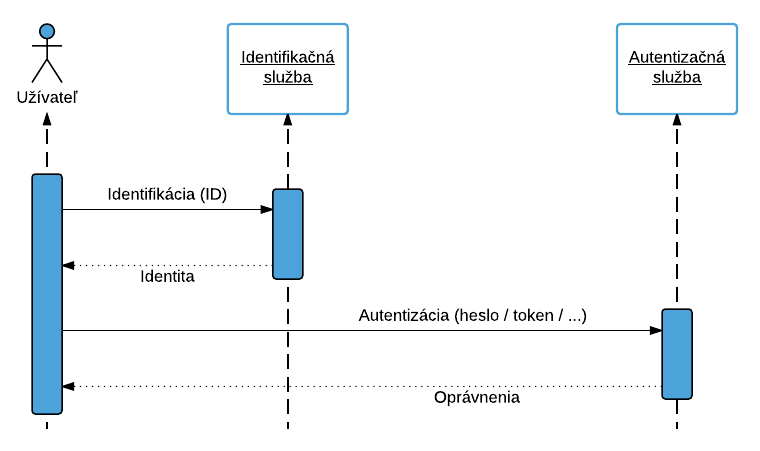
\includegraphics[width=.99\textwidth]{images/tech-app.png}
  \caption{Grafické znázornenie procesu identifikácie užívateľa na aplikačnej
  úrovni a jeho následnej autentizácie, zdroj: vlastné spracovanie}
  \label{fig:tech-app}
\end{figure}

\subsection{Výhody a nevýhody}
Identifikátory na aplikačnej úrovni sú veľmi jednoznačné a presné z hľadiska
priradenia účtu užívateľovi. Je pomocou nich preto následne možné presne
sledovať jeho akcie a manipulovať s privilégiami.

Tieto identifikátory sa však v abstrakcii komunikácie nachádzajú príliš vysoko,
preto nie je pomocou nich možné ovplyvniť napríklad DoS útoky popísané v
kapitole \ref{ch:dos}.

\section{Zhrnutie}
Na identifikáciu užívateľa, prípadne jeho zariadenia, sú v súčasnosti
používané rôzne techniky na rôznych vrstvách sieťovej infraštruktúry, od IP
adries sieťovej vrstvy, cez atribúty TCP protokolu, až po komplexné aplikačné
identifikátory. 

V praktickej časti tejto práce, ktorá sa zaoberá návrhom a implementáciou
unikátneho identifikátora, je použitá kombinácia informácií zo všetkých
spomínaných vrstiev (IP adresy, informácie z HTTP a TCP protokolu, ...) tak,
aby vznikol čo najpresnejší možný odtlačok aktivity jedného užívateľa.

\chapter{Tvorba unikátneho identifikátora}
\label{ch:footprint}
Hlavným cieľom a výstupom tejto práce je algoritmus definujúci jednoznačný
identifikátor užívateľa. Nasledujúca kapitola sa zaoberá práve popisom jeho
fungovania, štruktúry, použitých technológií a následnou implementáciou. Na
jeho tvorbu boli použité informácie HTTP a TCP protokolu popísané v
kapitolách \ref{ch:net-layers} a \ref{ch:existing}. Vďaka nim je algoritmus
schopný rozpoznať a priradiť aktivitu každému z používateľov hostiteľského
systému.

Princípom fungovania algoritmu je spúšťacia akcia, ktorou je prijatie HTTP requestu
hostiteľským serverom.\footnote{Hostiteľským serverom je typicky backendová
aplikácia, ktorá obsahuje implementáciu algoritmu ako nezávislý modul.} Na
základe každého takéhoto requestu je následne spustená jeho analýza a
porovnávanie. Výstupom algoritmu je miera podobnosti aktuálneho
requestu v podobe jeho vzdialenosti od najbližšieho podobného requestu
z databázy. Doplnkovou funkcionalitou je aj možnosť upozornenia hostiteľskej
aplikácie pri prekročení veľkého množstva podobných requestov od jedného používateľa.

\section{Popis Algoritmu}
Vo všeobecnosti pozostáva celý algoritmus z piatich hlavných, po sebe nasledujúcich krokov:
\begin{enumerate}
  \item Zachytenie prebiehajúceho requestu pred samotným spracovaním logikou hostiteľskej aplikácie.
  \item Zhromaždenie HTTP a TCP informácií daného spojenia.
  \begin{itemize}
    \item HTTP dáta sú parsované zo zachyteného requestu.
    \item TCP dáta poskytuje samostatný sieťový monitor.
  \end{itemize}
  \item Spracovanie a serializácia informácií do podoby objektu unikátneho odtlačku
  aktuálneho requestu.
  \item Analýza a nájdenie najbližšieho podobného identifikátora v databáze pomocou funkcie na
  hľadanie najmenšej vzdialenosti.
  \item Spracovanie výsledku v podobe vzdialenosti odtlačkov a následná reakcia.
  \begin{itemize}
    \item Ak ide o novú reláciu, pre identifikátor je vytvorený nový záznam v databáze s frekvenciou 1.
    \item V prípade, že miera podobnosti prekročila stanovený prah, nevytvára
    sa nový záznam. Frekvencia daného odtlačku v databáze je však zvýšená.
    \item Ak je frekvencia výskytu konkrétneho odtlačku veľmi vysoká existuje
    možnosť upozornenia hostiteľskej aplikácie.
  \end{itemize}
\end{enumerate}

\begin{figure}[h]
  \centering
    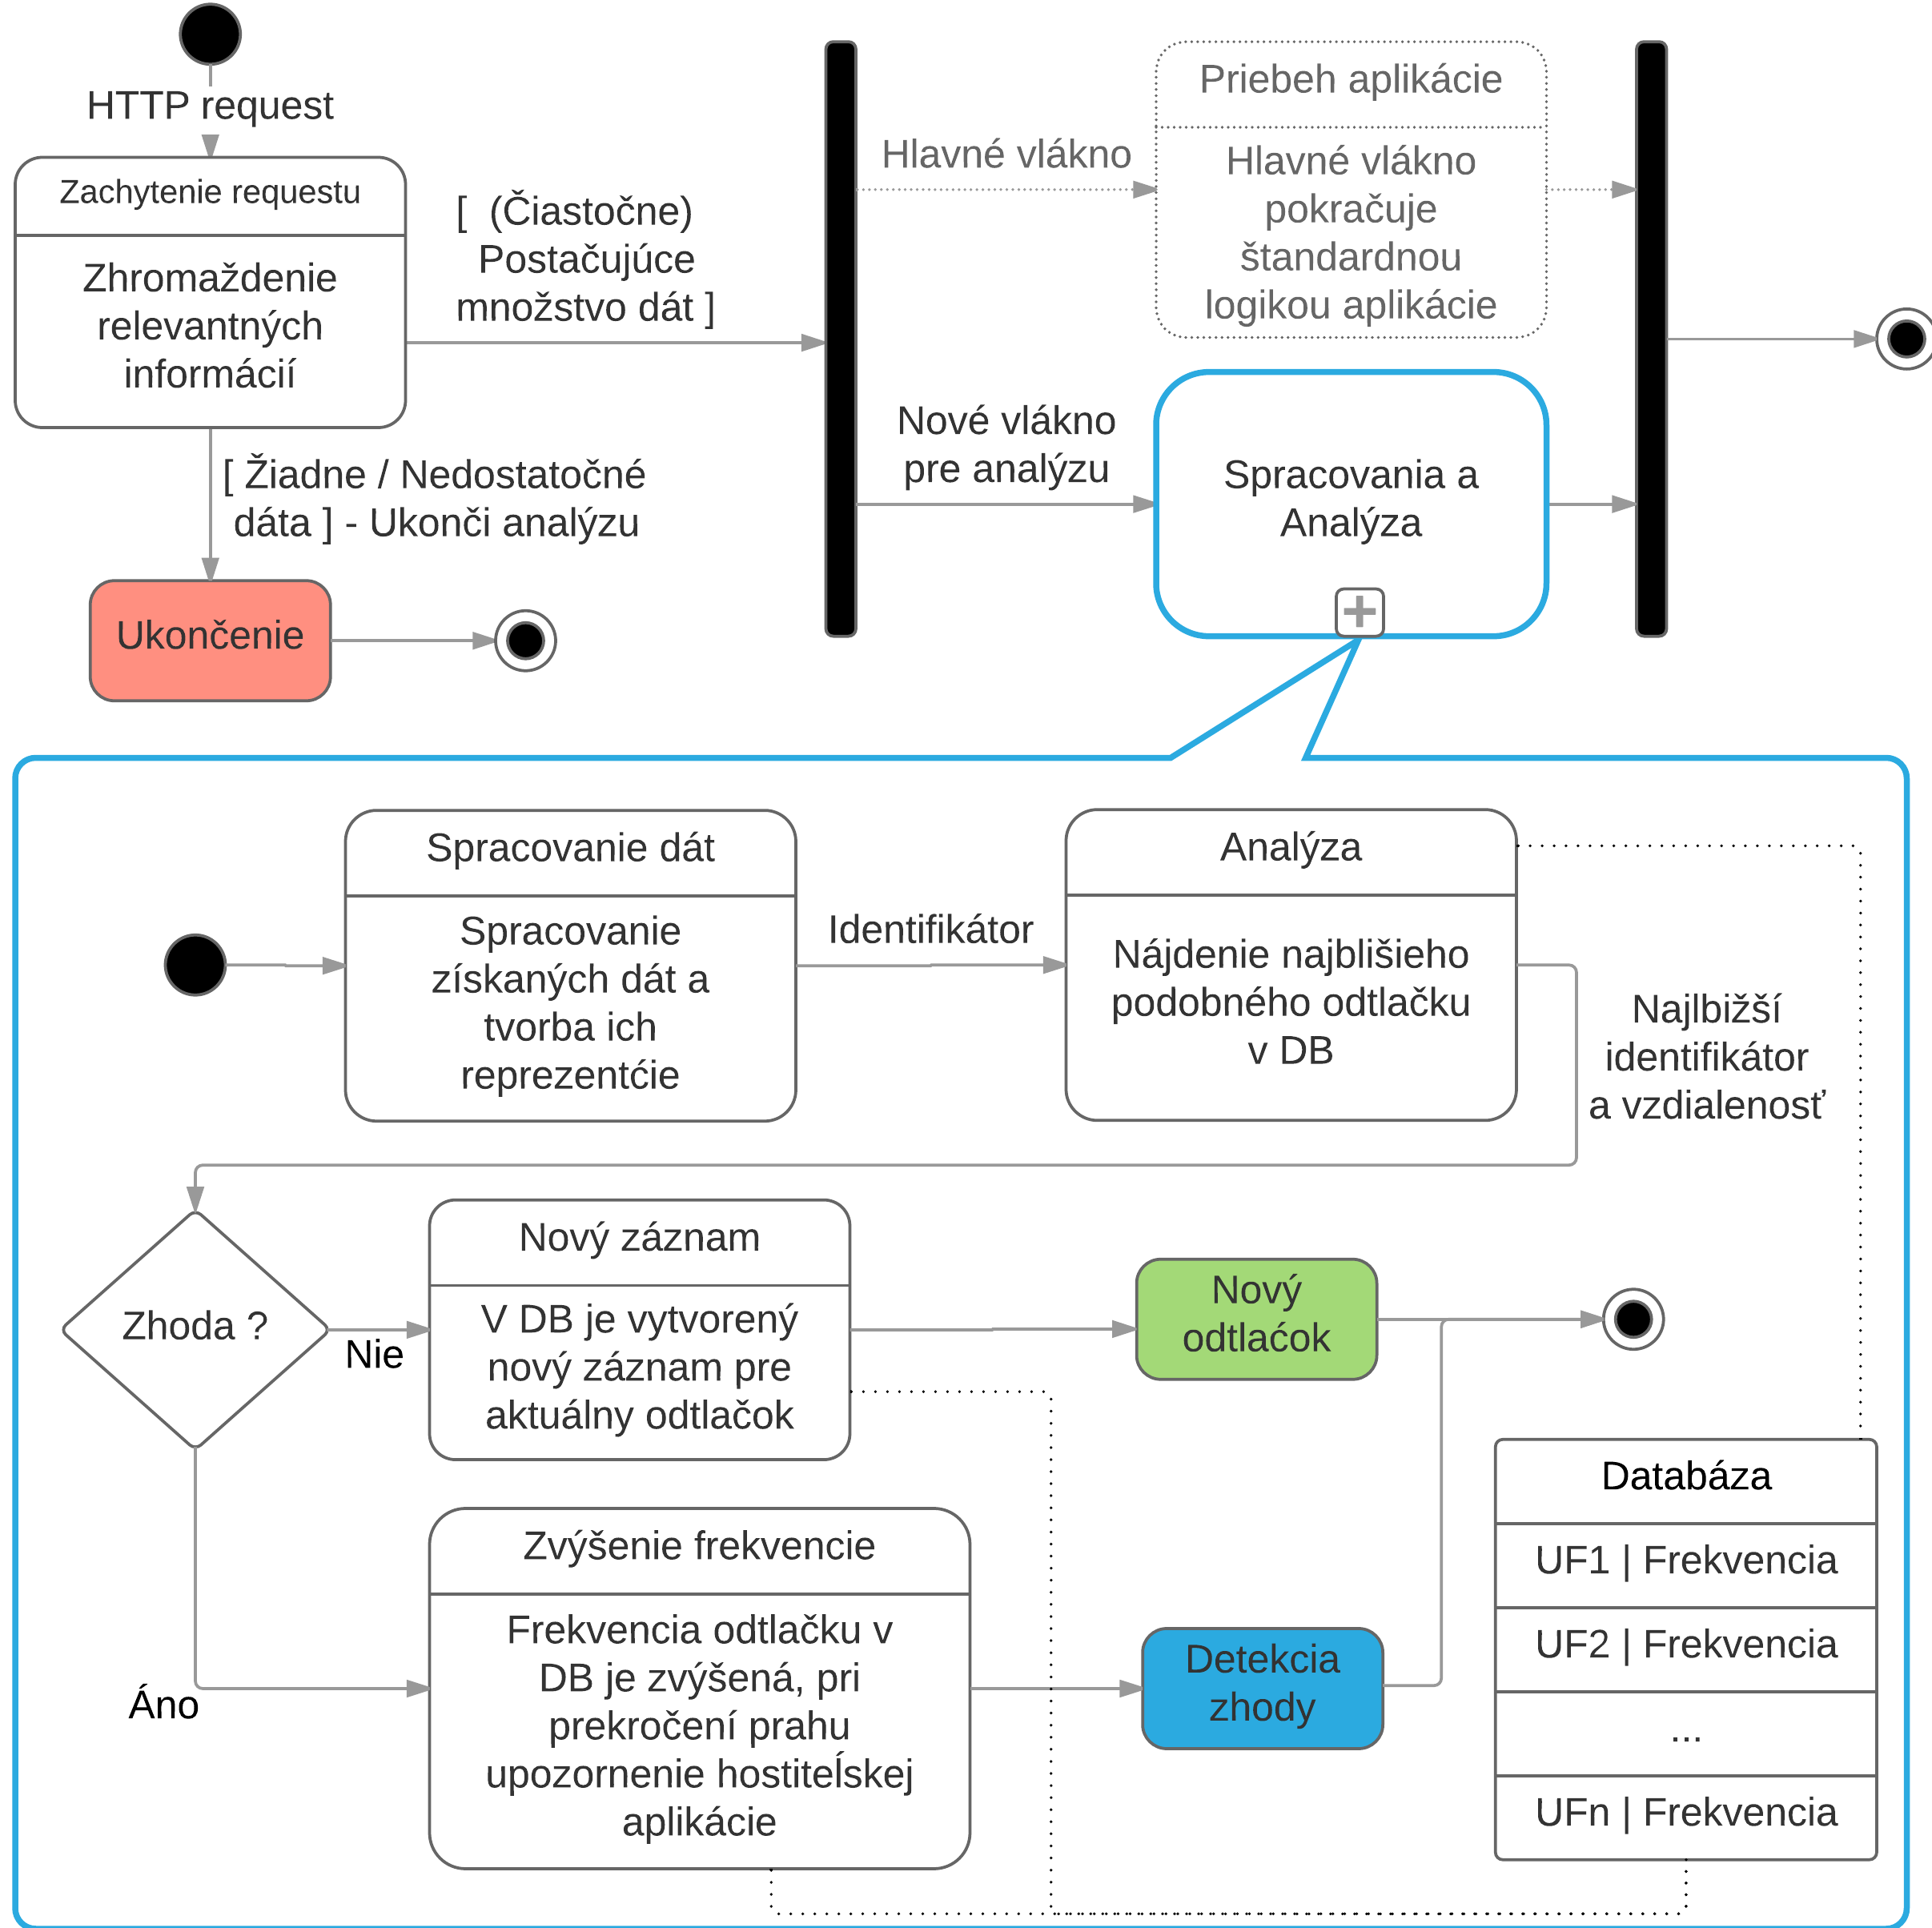
\includegraphics[width=.93\textwidth]{images/footprint-hl.png}
  \caption{Diagram znázorňujúci celý proces algoritmu spracovania requestu a
  hľadania podobnosti, zdroj: vlastné spracovanie}
  \label{fig:footprint-hl}
\end{figure}

Ako je podrobne znázornené na diagrame \ref{fig:footprint-hl}, analýzu spúšťa každý nový
HTTP request, na ktorý ďalej nadväzujú akcie tvorby a porovnávania
identifikátorov. Zároveň je pri štarte aplikácie spustené vlákno vykonávajúce
sieťovú analýzu transportnej vrstvy, ktorá uchováva informácie z niekoľkých
posledných spojení. Z týchto HTTP a TCP informácií je teda pre každý request
zostavený unikátny odtlačok - identifikátor \textit{(Unique Footprint - UFoo)}.
Aktuálny identifikátor je následne porovnávaný s každým odtlačkom v databáze.
Algoritmus na hľadanie najbližšieho suseda k nemu následne pomocou porovnávacej
funkcie nájde najbližší identifikátor. Podľa miery podobnosti ďalej
algoritmus určí, či ide o requesty jedného užívateľa, čo spôsobí zvýšenie jeho
frekvencie, alebo ide o nový odtlačok, pre ktorý vytvorí nový záznam.
Ako bolo popísané vyššie, jednou z dodatočných funkcionalít je aj upozornenie hostiteľskej aplikácie pri
prekročení limitu frekvencie requestov od jedného užívateľa, čo by mohlo
indikovať napríklad DoS, prípadne DDoS útok.

\section{Štruktúra identifikátora}
\label{s:footprint-structure}
Odtlačok aktivity užívateľa je teda kombináciou špecificky vybraných HTTP a TCP informácií.
Objekt sa skladá z dvoch častí - statických a relačných dát. Dôležitejšou z
nich sú takzvané statické dáta, ktoré slúžia porovnávacej funkcii na samotné
určenie vzdialenosti dvoch identifikátorov. Vzdialenosť vypočítaná touto
funkciou môže byť ďalej ovplyvňovaná vzťahmi relačných dát, ktoré riešia
špecifické aspekty vybraných informácií, ako napríklad určenie menej bezpečných
geo-zón geolokáciou IP adresy klienta.

\subsection{Statické dáta}
Statická časť identifikátora obsahuje väčšie množstvo dát, preto je
ukladaná a reprezentovaná v podobe reťazca. Skladá sa z nasledujúcich troch podčastí dát pre porovnávanie:
\begin{itemize}
    \item Statické hlavičky \textit{(Static headers)} - špecifické vopred
    vybrané a zoradené hodnoty HTTP hlavičiek, ako napríklad: \textit{authorization, cookie, content-length}, alebo
    \textit{user-agent}.
    \item Neznáme hlavičky \textit{(Unknown headers)} - ostatné hlavičky daného
    HTTP requestu, ktoré neboli použité ako statické.
    \item Atribúty - konkrétne informácie z HTTP a TCP protokolu, ako napríklad
    \textit{IP adresa, geo-lokácia}, alebo pre \textit{veľkosť TCP okna}.
\end{itemize}

Súhrnne znázorňuje všetky použité informácie jednotlivých kategórií statických dát schéma
\ref{fig:footprint-data-static}.

\begin{figure}[h]
  \centering
    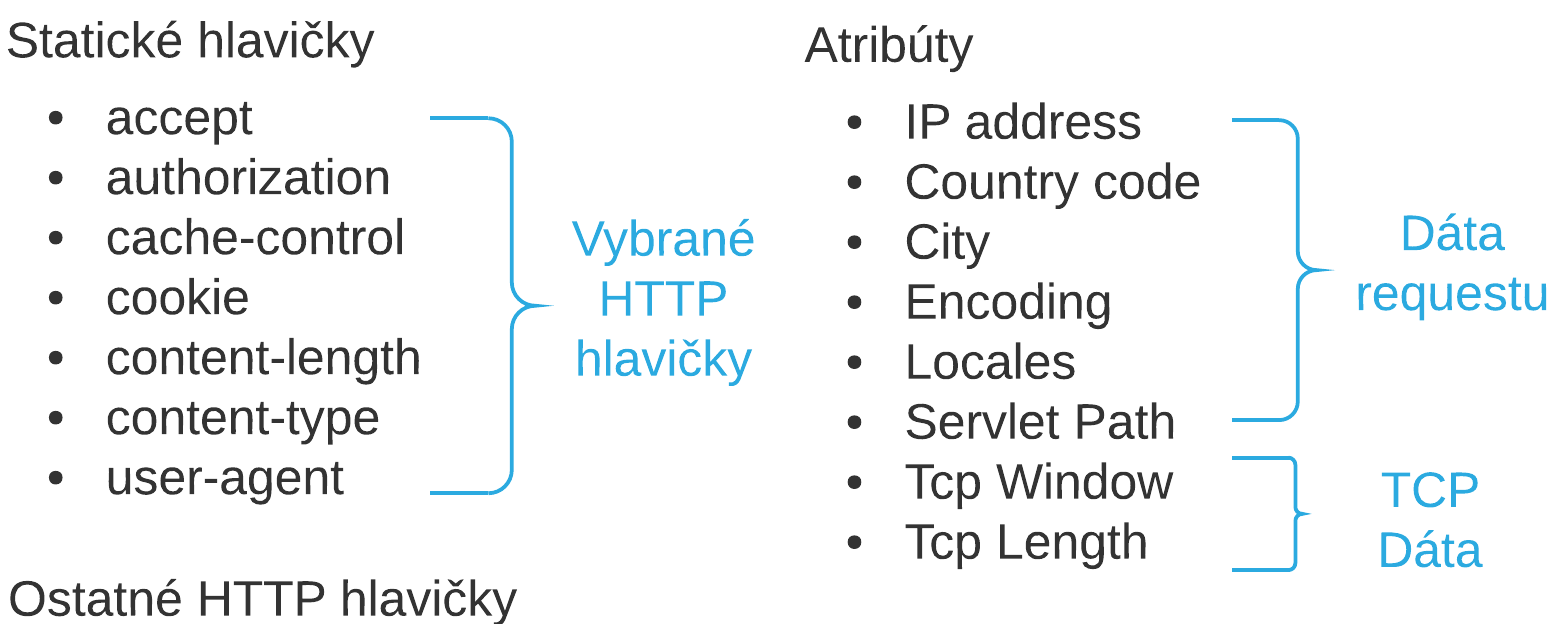
\includegraphics[width=.95\textwidth]{images/footprint-data-static.png}
  \caption{Detailný pohľad na štruktúru statických dát identifikátora, zdroj:
  vlastné spracovanie}
  \label{fig:footprint-data-static}
\end{figure}

Každá z týchto informácii má pri použití v porovnávacej funkcii svoj účel a
konkrétnu váhu, ktorá určuje jej dôležitosť. Veľmi podstatný je napríklad obsah statických hlavičiek. Naopak
váha hodnôt TCP okna je v porovnaní s IP adresou a geolokáciu menšia, môže však
hrať rolu u veľkého množstva requestov. Podrobnejšie sa porovnávacej funkcií a
spôsobu výpočtu podobnosti jednotlivých parametrov venuje podkapitola \ref{ss:distance-function}.

\subsection{Relačné dáta}
Relačné dáta neslúžia na porovnávanie a hľadanie podobných hodnôt. Ich účelom
je ošetriť špeciálne prípady u informácií, ktoré si to vyžadujú. Takýchto
informácií nie je mnoho, preto nie je nutné ich komprimovať a serializovať do podoby reťazca ako
dáta statické.
Ide teda o objekt obsahujúci nasledujúce položky:
\begin{itemize}
    \item Timestamp - presný čas nadviazania spojenia aktuálnej relácie.
    \item Geolokáciu - krajina pôvodu určená na základe IP adresy klienta.
    \item Relačné hlavičky - HTTP hlavičky, ako napríklad
    \textit{forwarded}, alebo \textit{x-csrf-token}. 
\end{itemize}

Jednotlivé položky sú vyhodnocované samostatne a ich výsledky sú aplikované na
vzdialenosť vrátenú algoritmom pre nájdenie podobnosti. Napríklad pri veľmi
malom časovom rozdiele porovnávaných requestov, je ich vzdialenosť dodatočne
znížená. U geolokácie môže byť zmena parametra výpočtu dosiahnutá po vyhodnotení requestu
klienta z krajiny s najčastejším pôvodom DoS útokov, akými sú napríklad: Čína,
Kórea, alebo Rusko.

\subsection{Variabilita štruktúry dát}
Štruktúra statických a relačných dát odtlačku je v aplikácii kalibrovaná
pre čo najpresnejšie určenie podobnosti requestov od jedného používateľa.
Samozrejme je však možné ju v budúcnosti obmieňať, prípadne pridávať do nej
nové informácie.

\section{Algoritmus hľadania podobnosti}
\label{s:similarity-search}
Ako bolo spomínané v predchádzajúcich odsekoch, hlavnou funkcionalitou procesu identifikácie je
algoritmus na určenie podobnosti a hľadanie najbližšieho suseda aktuálne
spracovávaného identifikátora. 

Vstupom pre algoritmus je teda tento odtlačok
spolu s množinou obsahujúcou odtlačky doteraz analyzovaných requestov.

Po
inicializácii a načítaní vstupných parametrov je na každú dvoji-cu odtlačkov
aplikovaná funkcia pre výpočet ich vzdialenosti, ktorá vráti hodnotu v rozmedzí
od nula do jedna. Pre totožné odtlačky je vzdialenosť nulová, naopak u
odtlačkov, ktoré sa líšia v mnohých parametroch sa hodnota blíži k jednej.
Funkcia postupne porovnáva a zohľadňuje jednotlivé hodnoty statickej časti
identifikátora podľa ich váhy a miery podobnosti. Detailným popisom fungovania
tejto funkcie sa zaoberá podkapitola \ref{ss:distance-function}. 

Po spracovaní
výsledkov algoritmus nájde najbližší identifikátor, ktorý spolu s jeho
vzdialenosťou vráti ako výstup na ďalšie spracovanie a prípadnú úpravu
relačnými dátami.

Nasledujúci pseudo-kód teda formálne popisuje tento algoritmus a jeho prácu s
výsledkami funkcie na výpočet vzdialeností:
\begin{lstlisting}[basicstyle=\footnotesize, language=Ruby, mathescape]
algorithm get-nearest-neigbour is
    input: UFooEntity uFooEntity
           UFooEntity[] allStockItems
    output: Result<int distance, UFooEntity nearestNeigbour>

    minDistance $\leftarrow$ MAX_INT;
    nearestneigbour $\leftarrow$ null;

    for each stockUFooEntity in allStockItems do

        acctualDistance $\leftarrow$ getDistance(uFooEntity.staticData,
                       stockUFooEntity.staticData);

        # Addition analysis - manual checks based on Relation Data
        # Possibly can SLIGHTLY afffect distance 

        if acctualDistance < minDistance then
            minDistance $\leftarrow$ acctualDistance;
            nearestneigbour $\leftarrow$ stockUFooEntity;
        end if
    
    return Result<minDistance, nearestneigbour>
\end{lstlisting}

\subsection{Použité postupy}
Pred samotným popisom funkcie pre výpočet vzdialeností odtlačkov je nutné
vysvetliť techniky a pojmy, s ktorými tento algoritmus pracuje. Konkrétne ide
okrem porovnávania komprimovaných reťazcov pre jednoduché atribúty, najmä o 
určenie miery podobnosti množín pomocou výpočtu takzvaného
\textit{Jaccardovho} indexu.

\subsubsection{Jaccardov index}
Výpočet Jaccardovho koeficientu, taktiež známy ako podiel prieniku a 
zjednotenia, je funkcia pôvodne popísaná Paulom Jaccardom, ktorá slúži na
porovnanie podobnosti a rozdielov testovaných množín. Jaccardov koeficient teda
meria mieru podobnosti medzi dvoma konečnými množinami. Matematicky je
definovaný ako podiel veľkostí zjednotenia a prieniku týchto množín:

\begin{equation}
 J(A,B) = {{|A \cap B|}\over{|A \cup B|}} = {{|A \cap B|}\over{|A| + |B| - |A \cap B|}}
\end{equation}

V prípade, že sú obe množiny prázdne \textit{J(A,B) = 1}.
Jaccardova vzdialenosť, ktorá naopak určuje rozdielnosť dvoch množín, je
doplnkom k Jaccardovmu koeficientu. Počíta sa teda odrátaním jeho hodnoty od
jednotky, prípadne ako podiel, ktorého čitateľom je rozdiel zjednotenia s
prienikom a menovateľom je zjednotenie týchto množín:

\begin{equation}
 d_J(A,B) = 1 - J(A,B) = { { |A \cup B| - |A \cap B| } \over |A \cup B| }
\end{equation}

\begin{equation}
 0\le J(A,B)\le 1
\end{equation}

\begin{figure}[h]
  \centering
    
\includegraphics[width=.99\textwidth]{images/footprint-jacc-sets.png}
  \caption{Znázornenie prieniku a zjednotenia množín pre výpočet Jaccardovho
  koeficientu, zdroj: ??}
  \label{fig:footprint-jacc-sets}
\end{figure}

\subsubsection{Porovnávanie atribútov}
Pri porovnávaní konkrétnych reťazcov u HTTP hlavičiek, alebo atribútov, ako
napríklad \textit{servletPath}, alebo \textit{locales}, sú tieto hodnoty pred
porovnaním komprimované. Konkrétne ide o odstránenie nadbytočných bielych
znakov a symbolov, ktoré by mohli pri porovnaní spôsobovať nepresnosti. Rovnaké
pravidlá sú použité aj pri porovnávaní položiek pri výpočte Jaccardovho indexu.

\subsection{Funkcia na výpočet vzdialenosti}
\label{ss:distance-function}
Vstupom pre funkciu na výpočet vzdialenosti sú teda vždy dve reprezentácie
identifikátorov, konkrétne hodnoty v ich statickej časti. Výsledná vzdialenosť
je počítaná ako doplnok váženého priemeru podobností troch podčastí týchto dát
nasledovne:

\begin{itemize}
	\item Ako prvý je spočítaný Jaccardov koeficient pre statické hlavičky.
	\item Následne algoritmus použije Jaccardov index aj pre výpočet podobnosti
	zvyšných hlavičiek.
	\item Nakoniec je vypočítaná miera podobnosti jednotlivých atribútov. 
\end{itemize}

Každá z týchto častí je pri následnom sčítaní vážená vlastnou konštantou.
Zároveň má vlastnú váhu každý z atribútov tretej časti. Konkrétnu kalibráciu
váh jednotlivých položiek znázorňuje schéma \ref{fig:footprint-distance-cal}.

\begin{figure}[H]
  \centering
    
\includegraphics[width=.93\textwidth]{images/footprint-distance-cal.png}
  \caption{Príklad kalibrácie váh jednotlivých parametrov statickej časti
  odtlačku pre výpočet vzdialenosti, zdroj: vlastné spracovanie}
  \label{fig:footprint-distance-cal}
\end{figure}

Kľúčovú rolu pri výpočte samozrejme zohráva práve spomínaná kalibrácia váh a parametrov tohto
algoritmu. Nasledujúci pseudo-kód formálne popisuje funkciu výpočtu vzdialenosti a jej fungovanie:

\vspace{6mm}
%noindent\rule{13cm}{0.4pt}
\begin{lstlisting}[basicstyle=\footnotesize, language=Ruby, mathescape=true]
algorithm get-distance is
    input: String actualData
           String stockEntityData
    output: double distance

    if actualData = stockEntityData
        return 0
    end if

    # Compute weighted Jaccard for static headers
    jaccardStaticHeaders 
    	$\leftarrow$ jaccardIndex(actualData.staticHeaders, 
    	                stockEntityData.staticHeaders);
    jaccardStaticHeaders 
    	$\leftarrow$ jaccardStaticHeaders * SH_WEIGHT;

    # Compute weighted Jaccard for unknown headers
    jaccardUnknownHeaders 
    	$\leftarrow$ jaccardIndex(actualData.unknownHeaders,
    	                stockEntityData.unknownHeaders);
    jaccardUnknownHeaders 
    	$\leftarrow$ jaccardUnknownHeaders * UH_WEIGHT;

    # Compare values of remaining attributes by similarValue
    # function. Every of this attributes will have sub-weight
    # which will be computed in attributesIndex.
    isSameIp 
    	$\leftarrow$ similarValue(actaulData.IP, stockEntityData.IP)
    	* IP_SUB_WEIGHT;
    isSameCountry 
    	$\leftarrow$ similarValue(actaulData.country, 
    	                stockEntityData.country)
    	* COUNTRY_SUB_WEIGHT;
    ...
    isSameLength 
    	$\leftarrow$ similarValue(actaulData.length, 
    	                stockEntityData.length)
    	* LENGTH_SUB_WEIGHT;

    attributesIndex 
    	$\leftarrow$ $\sum$(isSameIp, isSameCountry, ..., isSameLength) 
    	 / $\sum$(IP_SUB_WEIGHT, COUNTRY_SUB_WEIGHT,
    	     ..., LENGTH_SUB_WEIGHT);
    attributesIndex 
    	$\leftarrow$ attributesIndex * ATTR_WEIGHT

    similarity 
    	$\leftarrow$ $\sum$(jaccardStaticHeaders,  jaccardUnknownHeaders,
    	     attributesIndex) 
    	 / $\sum$(SH_WEIGHT, UH_WEIGHT, ATTR_WEIGHT)

    return 1 - similarity;
\end{lstlisting}

Hodnoty podobností jednotlivých častí sú teda násobené pridelenými váhami a
sčítané. Podielom súčtov týchto hodnôt a ich možných váh je následne vypočítaný
koeficient podobnosti statických dát vstupných identifikátorov. Výstupom 
funkcie je vzdialenosť, ktorá je doplnkom k tomuto koeficientu.

\section{Implementácia}
Súčasťou tejto práce je okrem návrhu algoritmu aj jeho implementácia v jazyku
Java. Ide o presnú implementáciu funkcionality popísanej v predchádzajúcich
podkapitolách. Knižnica samotná je čo najuniverzálnejšia a nezávislá na
konkrétnom \textit{frameworku}, či technológii. Po vložení jej závislosti do
hostiteľského projektu sama detekuje prístupové metódy a zachytáva jednotlivé
HTTP requesty pre ďalšie spracovanie. Zároveň pri spustení, ak je to možné,
začne monitorovať sieť pre doplnenie informácií z TCP protokolu.

\subsection{Použité technológie}
Pre korektnú implementáciu funkcionality celého algoritmu bolo nutné použitie
mnohých špecifických technológií, od knižnice pre monitoring TCP paketov, až po
geolokáciu IP adries. Nasledujúce odseky popisujú najdôležitejšie z nich.

\subsubsection{Aspektovo-orientované programovanie}
Aspektovo-orientované programovanie (ďalej len AOP) je paradigma určená k
zvýšeniu modularity kódu bez narúšania prirodzeného behu aplikácie. Ide o 
pridanie novej funkcionality k už existujúcemu kódu, bez nutnosti modifikácie
pôvodného zdroja. Namiesto toho je osobitne definovaný takzvaný prístupový bod,
ktorý pridá požadovanú funkcionalitu na vopred určené miesto.

V implementačnej časti je AOP, konkrétne knižnica \textit{AspectJ}, použitá pre
injektovanie jednotlivých prístupových metód hostiteľskej aplikácie a následné
odchytávanie informácií z ich HTTP requestov. Je tak možné vytvoriť prístupové
body pre ľubovoľný z používaných \textit{frameworkov}, či prístupov. Momentálne, na
testovacie účely, implementácia obsahuje prístupový bod pre metódy so
\textit{Springovou} anotáciou \textit{@RestController}. Nie je však problém
rozhranie rozšíriť o akýkoľvek existujúci, či vlastný prístupový bod. Ďalšou z 
výhod tohto prístupu je asynchrónnosť celého výpočtu. Po zachytení informácií
z HTTP requestu je proces ich spracovania vykonávaný v novom vlákne. Logika
hostiteľskej aplikácie tak nie je ničím zdržovaná a môže pokračovať štandardným
spôsobom.

\subsubsection{Sieťová analýza}
Pri štarte hostiteľskej aplikácie, je štandardne jedným z modulov v samostatnom
vlákne spustený monitoring, analýza a parsovanie TCP paketov. Pre prístup k
týmto informáciám je využívaná knižnica \textit{libpcap} a program
\textit{tcpdump}. Samozrejme tieto možnosti je nutné vopred povoliť na
hostiteľskom serveri, preto existuje možnosť aplikáciu používať aj bez
monitorovania sieťovej aktivity. Výpočty vzdialeností identifikátorov, ktoré
tieto informácie obsahujú sú však presnejšie a produkujú menej falošne
pozitívnych detekcií.

\subsubsection{IP Geolokácia}
Ako bolo popísané v sekcii \ref{s:footprint-structure}, jedným z atribútov, ktoré sú posudzované pri
vyhodnotení podobnosti identifikátorov je geolokácia klienta. Konkrétne ide o
krajinu, prípadne mesto, určené na základe jeho IP adresy. Zdrojom týchto
informácií je databáza poskytnutá službou \textit{MaxMind GeoIP}.

Okrem tejto databázy systém používa aj statický zoznam menej bezpečných zón.
Ide o konkrétne krajiny, ktoré sú najčastejším pôvodcom DoS a DDoS útokov. Ich
detekcia môže mať za následok napríklad zníženie prahu pre upozornenie
hostiteľskej aplikácie pri prekročení väčšieho množstva podobných odtlačkov.

\subsection{Funkcionalita a štruktúra kódu}
Celá akcia spracovania requestu začína v triede \textit{Injector}. Táto trieda
obsahuje prístupové body AOP pre jednotlivé metódy hostiteľskej aplikácie.
Zároveň slúži na správu závislostí a inicializáciu \textit{singleton} vlákna
triedy \textit{PacketStream}. \textit{PacketStream} a ostatné pomocné triedy
balíka \textit{endpoint.collector.tcp} zabezpečujú, ak je to možné, parsovanie a 
správu prijatých TCP paketov. Tieto sú následne dostupné ako mapa posledných
\textit{n} zachytených paketov v podobe množiny objektov triedy \textit{TCPFootprint} a ich IP
adries.

Z Injectora dáta pokračujú vždy v samostatnom vlákne na spracovanie triedou
\textit{RequestHandler} a ostatnými triedami balíka
\textit{endpoint.collector.http}. Ich účelom je extrahovať potrebné HTTP
informácie, ktoré sú následne reprezentované triedou \textit{HTTPFootprint}.
\footnote{Štruktúra tried \textit{HTTPFootprint} a \textit{TCPootprint} je dostupná v
prílohe \ref{fig:appendix-structure}.}

Ďalej už s reprezentáciami \textit{HTTPFootprint} a \textit{TCPFootprint}
pracuje trieda \textit{UFooProcessor}. Táto trieda obsluhuje hlavnú logiku
analýzy podobnosti aktuálne spracovávaného requestu s ostatnými identifikátormi
v databáze. \textit{UFooProcessor} pomocou metód triedy \textit{Serializer} spracuje informácie do
konečnej podoby objektu \textit{UFooEntity}, ktorý je reprezentáciou samotného
unikátneho identifikátora. \textit{UFooEntity} obsahuje všetky extrahované
statické a relačné dáta.

Najdôležitejšou časťou celého procesu je však analýza podobnosti vykonávaná triedou
\textit{FootprintSimilairtyService}, ktorá implementuje algoritmus hľadania
najbližšieho suseda formálne popísaný v sekcii \ref{s:similarity-search}. Jej
metódy \textit{getNearestNeighbour},  \textit{computeDistance} a
\textit{jaccardIndex} teda spočítajú konečný výsledok v podobe vzdialenosti a
najbližšieho podobného identifikátora z databázy.

Na základe tohto výsledku sa následne \textit{UFooProcessor} rozhodne, či ide o
aktivitu neznámeho užívateľa a vytvorí pre aktuálny odtlačok nový záznam v
databáze, alebo ide o opakujúcu sa reláciu, čím zvýši jeho frekvenciu, prípadne
upozorní hostiteľskú aplikáciu na možné prekročenie jej limitu.

Celý priebeh spracovania a analýzy podobnosti reqestu je zároveň znázornený
sekvenčným diagramom v prílohe \ref{fig:appendix-impl-flow}.

Spracovanie a analýza dát z jednotlivých requestov prebieha asyn-chrónne,
aplikácia teda nemusí čakať na dokončenie a jej výsledok. V prípade hrozby je
samozrejme upozornená. 

Pre účely testovania a kalibrácie parametrov algoritmu obsahuje praktická časť práce okrem
knižnice samotnej aj príklad hostiteľskej aplikácie, v ktorej je knižnica
použitá. Tento server takisto poskytuje možnosť zobrazenia jednoduchých
štatistík z analýzy podobnosti.

\chapter{Test s reálnymi dátami}
\label{ch:data}
Algoritmus a jeho implementácia popísaná vyššie boli testované a kalibrované na
simulácií reálneho D-DoS útoku. \footnote{Všetky citlivé dáta, ako napríklad reálne IP
adresy boli agregované a anonymizované, aby nemohlo dôjsť k ich následnému
zneužitiu.} Nasledujúce odseky popisujú jednak priebeh tohto
útoku, ako aj priebeh a výsledky jeho simulácie. 

\section{Parametre útoku}
Útok, na ktorom je následná simulácia založená, bol pomerne rozsiahly a dobre
organizovaný. Celkovo trval 56 minút a zúčastnili sa ho klienti zo 136 rôznych
IP adries. V priebehu týchto 56 minút server prijal dohromady 1 345 446 requestov, pričom
všetky smerovali na rovnakú URL a jednu konkrétnu akciu. Jeho ďalším znakom je
pomerne malá diverzita obsahu HTTP hlavičiek. Príklady týchto hlavičiek
niektorých z requestov zobrazuje nasledujúca schéma: 

\begin{lstlisting}[basicstyle=\footnotesize, mathescape=true]
[
    "Connection": "keep-alive",
    "User-Agent": "Mozilla/5.0 (Windows NT 10.0; )...",
    "Content-Type": "application/json; charset=UTF-8",
    "Host": "sample-domain.com",
    "Accept": "application/json, text/javascript, q=0.01",
    "Origin": "http://sample-domain.com",
    "Cookie": "__gvf=DN-24; _be=DV1.2; SampleTool...",
    "Accept-Encoding": "gzip, deflate",
    "Referer": "http://sample-domain.com/pages/homepage...",
    "X-Requested-With": "XMLHttpRequest",
    "Accept-Language": "en-US,en;q=0.8"
]
\end{lstlisting}

Na tento útok bolo teda použité veľké množstvo zariadení, ktoré postupne
odosielali požadované dáta. Všetky requesty však obsahovali podobnú skupinu
HTTP hlavičiek, s rôznymi obmenami, čo pomohlo k jeho lepšej identifikácií.

\section{Parametre simulácie}
Simulácia vyššie popísaného útoku sa ho snažila čo najvernejšie napodobniť.
Samozrejme však nebolo možné uskutočniť ho v plnom rozsahu. Na testovací server
bola preto vytvorená štandardná záťaž v podobe 25 000 requestov. Tieto requesty
sa snažili svojim obsahom čo najvernejšie napodobniť reálnych používateľov a
ich aktivitu. Paralelne bol na server  v priebehu niekoľkých desiatok minút
odosielaný obsah simulujúci spomínaný D-DoS útok v rozsahu 13 454 requestov z
13 rôznych IP adries. Ostatné parametre pôvodného útoku a obsah HTTP hlavičiek
zostali zachované.

Účelom tejto simulácie bolo overiť správnosť fungovania algoritmu, najmä jeho
schopnosť identifikácie a rozlíšenia aktivity používateľov D-DoS útoku od
štandardných relácií.

\section{Interpretácia výsledkov}
Nasledujúce grafy zobrazujú výsledky simulovaného útoku v porovnaní z aktivitou
bežných užívateľov. Všetky výsledky, ako aj ich grafické znázornenie boli
produkované aplikáciou, používajúcou implementáciu knižnice pre účely testovania
algoritmu, ktorá je súčasťou praktickej časti práce.

\begin{figure}[H]
  \centering
    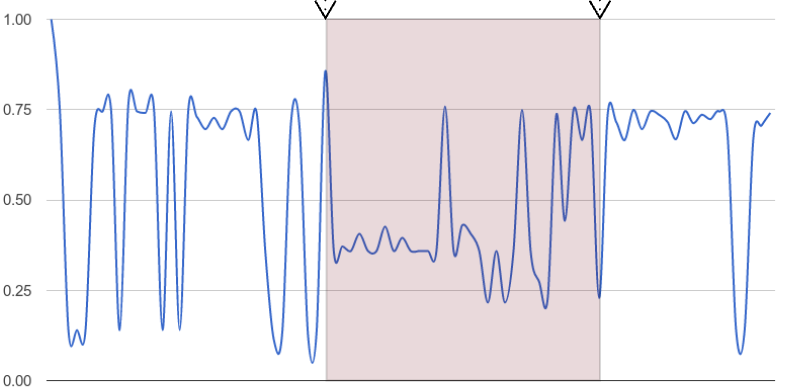
\includegraphics[width=.95\textwidth]{images/data-flow.png}
  \caption{Vzdialenosť reqestov simulácie, spolu z ohraničením začiatku a konca
  D-DoS útoku v čase, zdroj: implementačná časť práce}
  \label{fig:data-flow}
\end{figure}

Graf \ref{fig:data-flow} znázorňuje výsledky výpočtu vzdialeností jednotlivých
requestov\footnote{Pre účely lepšej čitateľnosti je počet vzdialeností, z
ktorých bol graf rendrovaný redukovaný. Výsledkom je teda aproximácia
jednotlivých vzdialeností simulácie v čase} v čase. Vyznačený úsek poukazuje na
začiatok a koniec simulovaného D-DoS útoku.

Histogram \ref{fig:data-histogram} ďalej zobrazuje presné rozloženie počtu
vzdialeností celej simulácie. Zároveň farebne rozlišuje vzdialenosti vypočítané
pre requesty D-DoS útoku od vzdialeností reálnych užívateľov. 

\begin{figure}[h]
  \centering
    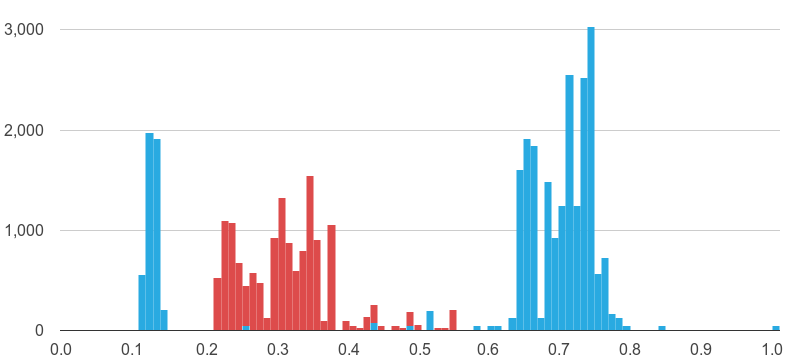
\includegraphics[width=\textwidth]{images/data-histogram.png}
  \caption{Histogram počtu vzdialeností requestov simulácie. Modrá farba
  reprezentuje vzdialenosti reálnych užívateľov, červená aktivitu D-DoS útoku,
  zdroj: implementačná časť práce}
  \label{fig:data-histogram}
\end{figure}

\begin{figure}[h]
  \centering
    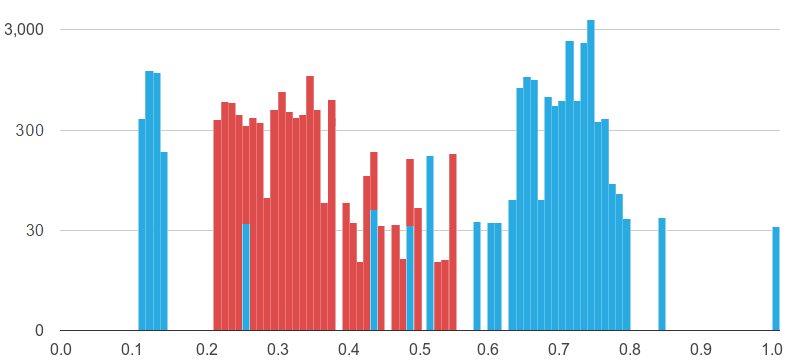
\includegraphics[width=\textwidth]{images/data-histogram-log.png}
  \caption{Histogram počtu vzdialeností requestov simulácie s použitím logaritmickej
  osi \textit{y}, zdroj: implementačná časť práce}
  \label{fig:data-histogram-log}
\end{figure}

\section{Zhrnutie}
Z výsledkov simulácie, najmä z výsledkov zobrazených v histograme
\ref{fig:data-histogram} je možné vidieť, že aktivitu requestov D-DoS útoku je
možné odlíšiť od aktivity reálnych používateľov meraním vzdialenosti
jednotlivých requestov. Zatiaľ čo vzdialenosti simulácie aktivity reálnych
užívateľov sa pohybujú vo väčšine prípadov v intervaloch \textit{<0.1,0.15>} a \textit{<0.6,0.8>},
väčšina vzdialeností simulácie aktivity D-DoS útoku sa pohybuje v intervale
\textit{<0.2,0.4>}. Zároveň existuje interval \textit{<0.4,0.6>} v ktorom sa v menšom
množstve oba typy prelínajú. Pre lepšie znázornenie stredného intervalu používa
histogram \ref{fig:data-histogram-log} logaritmickú os \textit{y}.
Podľa týchto údajov je teda možné kalibrovať aj prah pre
upozornenie hostiteľskej aplikácie na možnú hrozbu. 

\chapter{Záver}
Výsledky testov s reálnymi dátami dokázali funkčnosť algoritmu a jeho schopnosť
identifikácie užívateľov aj počas trvania simulácie prebiehajúceho DoS útoku.

Tieto výsledky sú však do istej miery aj pomerne prekvapivé. Pôvodná myšlienka
odhalenia requestov DoS útoku totiž počítala s veľkým počtom nízkych výsledných
vzdialeností u útočníka a vysokých vzdialeností u bežnej záťaže. 

Reálne však, ako je možné vidieť na histograme \ref{fig:data-histogram},
simulácia requestov reálnych užívateľov vykazovala maximá u okrajových hodnôt
vzdialeností a simulácia requestov DoS útoku u stredných hodnôt vzdialeností. 

Dôvodom tohto rozloženia je zrejme práve spôsob, akým útočník na rozdiel od
bežných užívateľov so serverom komunikoval. Bežní užívatelia totiž zasielali
navzájom pomerne rozdielne requesty, pričom requesty jedného užívateľa sa v jeho
relácii na seba podobali. To spôsobilo ich rozloženie do okrajových hodnôt
vzdialeností. Útočník ale celý čas používal jeden druh requestu, ktorý však
neustále obmieňal. Preto je rozloženie jeho vzdialeností v stredných hodnotách
škály. 

Na základe týchto výsledkov je teda možné nastaviť prahy pre určenie útoku
práve v intervale stredných vzdialeností útočníka, podľa výsledkov simulácie.

Táto problematika ma veľmi zaujala, preto prácu plánujem ďalej rozvíjať,
a dopĺňať o ďalšiu zaujímavú funkcionalitu od možnosti zdieľania
databázy odtlačkov, až po zlepšenie sledovania a použitia TCP informácií.

\makeatletter\thesis@blocks@clear\makeatother
\phantomsection %% Print the index and insert it into the
\addcontentsline{toc}{chapter}{\indexname} %% table of contents.
\printindex

\appendix %% Start the appendices.

\chapter{Sekvenčný diagram znázorňujúci priebeh spracovania reqestu}
\label{fig:appendix-impl-flow}
\begin{figure}[H]
  \centering
    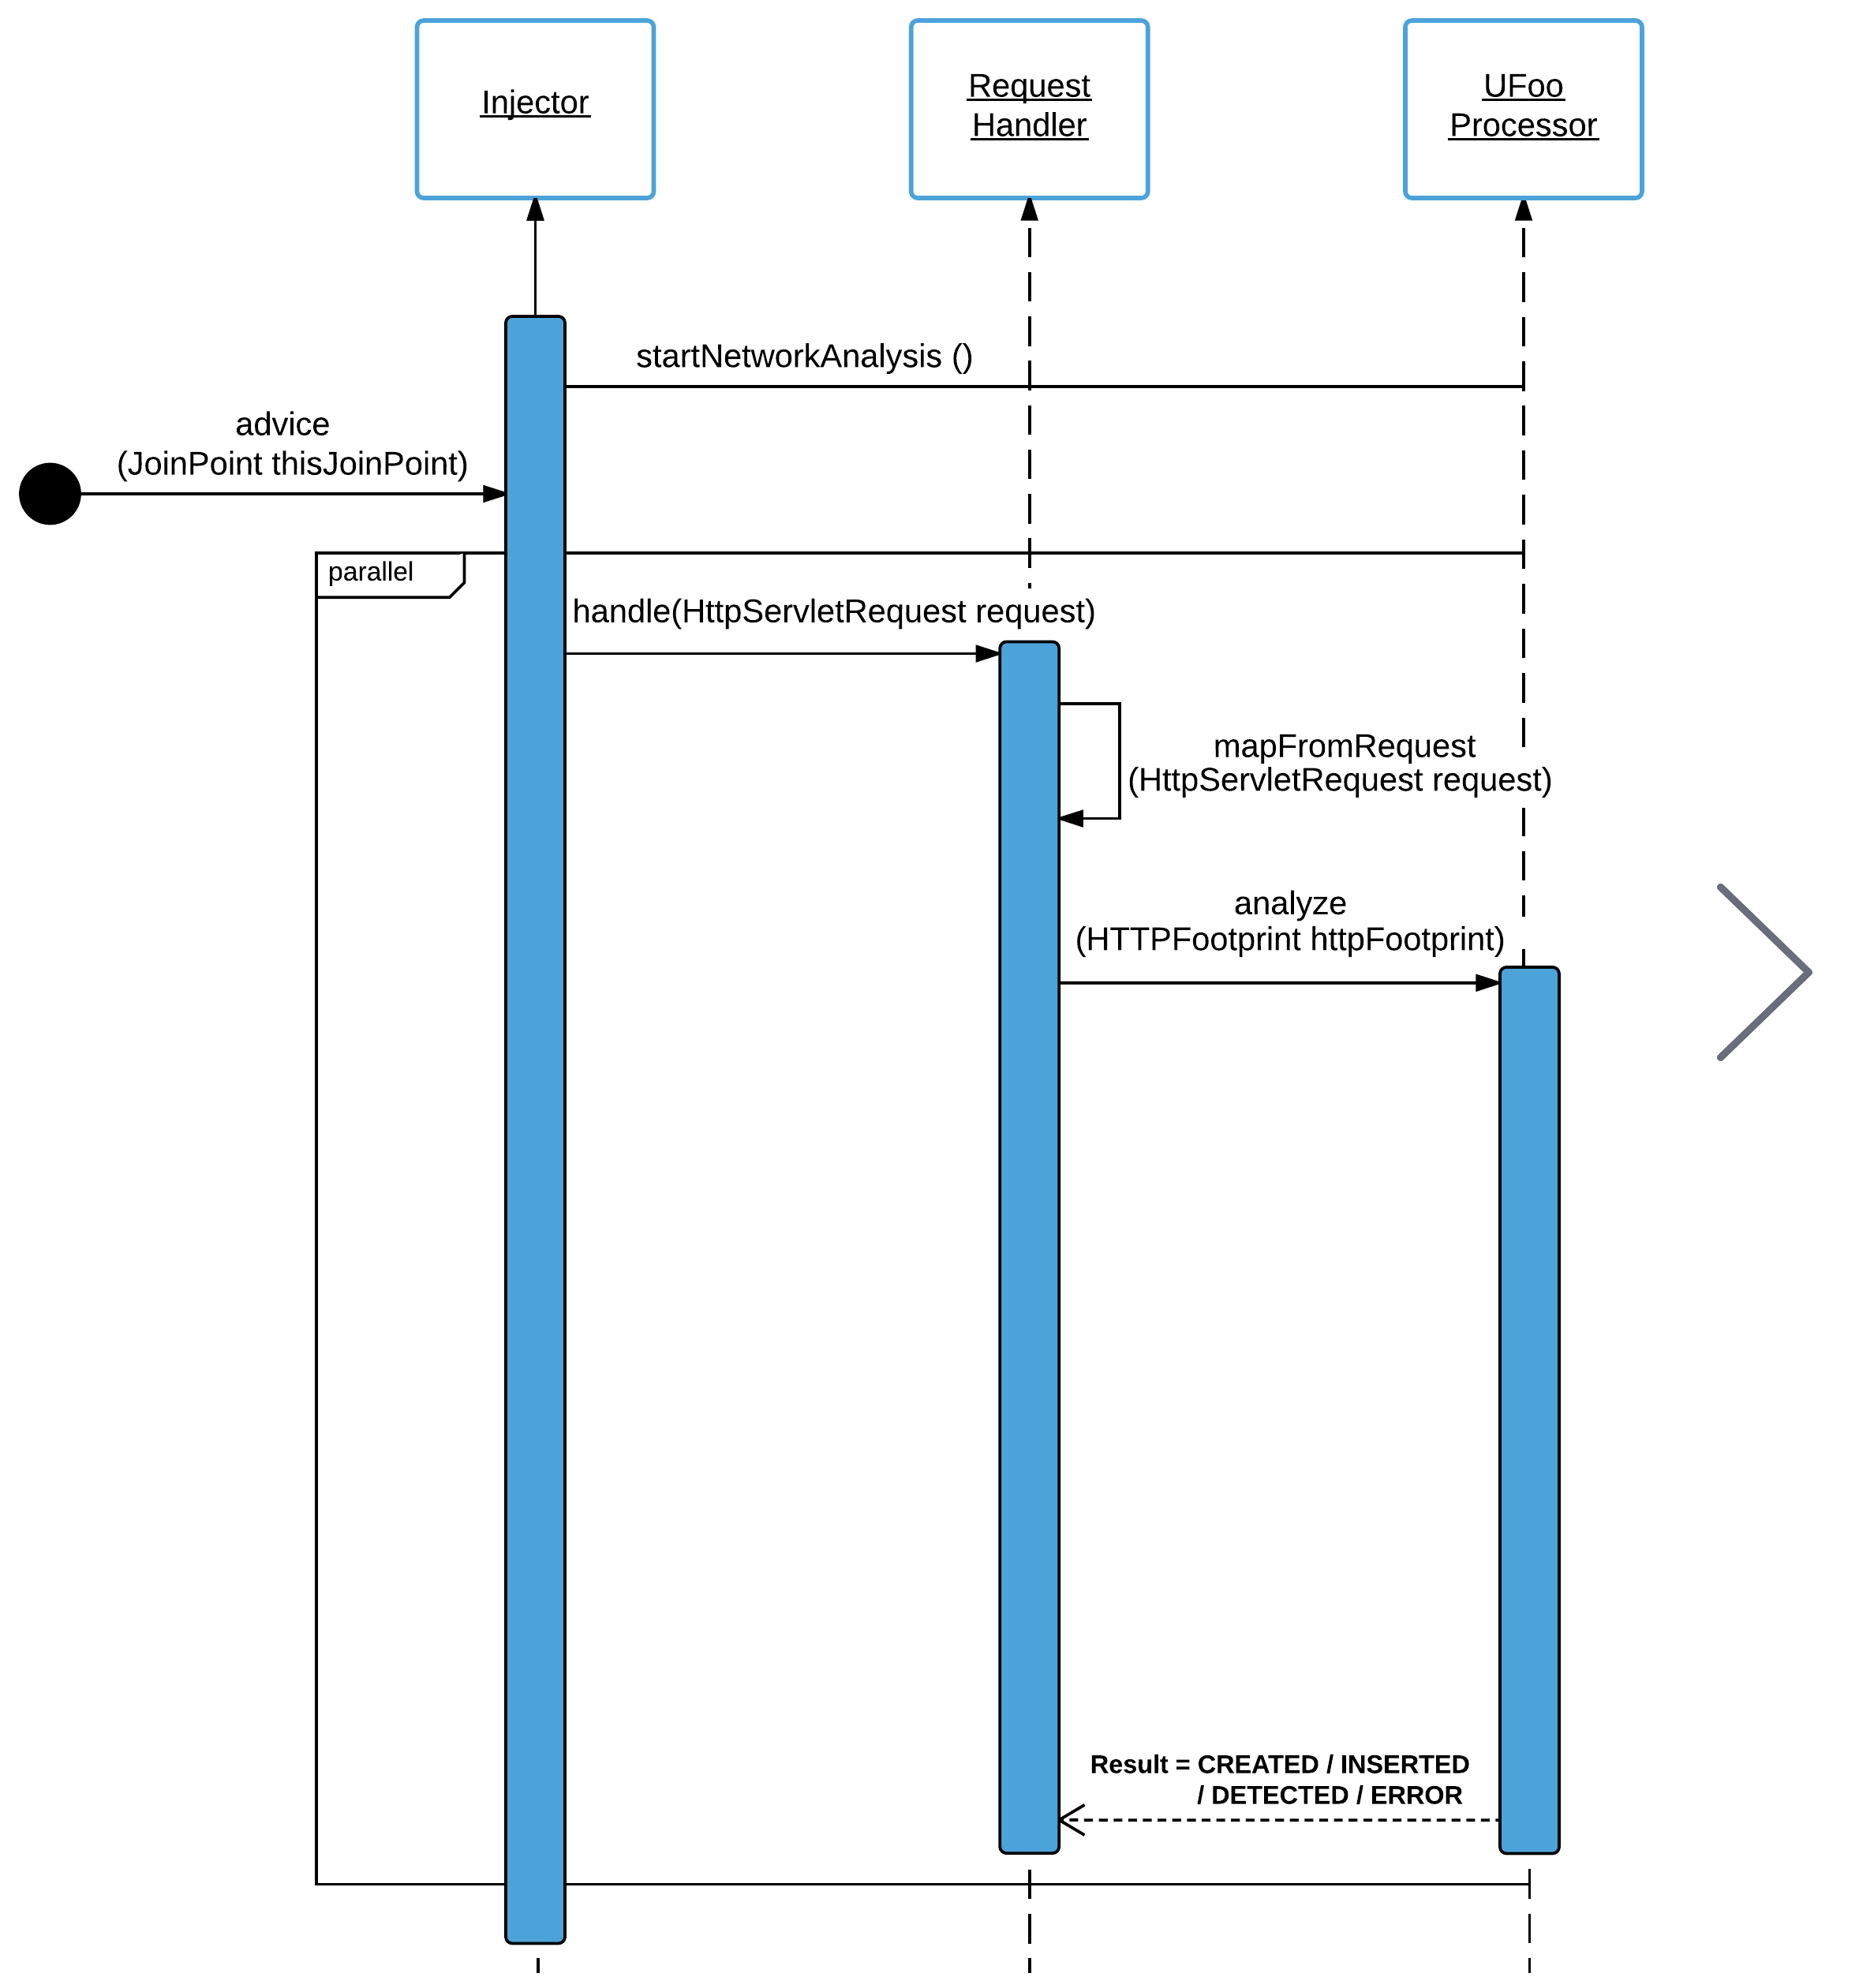
\includegraphics[width=1\textwidth]{images/footprint-impl-flow-1.png}
\end{figure}
\begin{figure}[h]
  \centering
    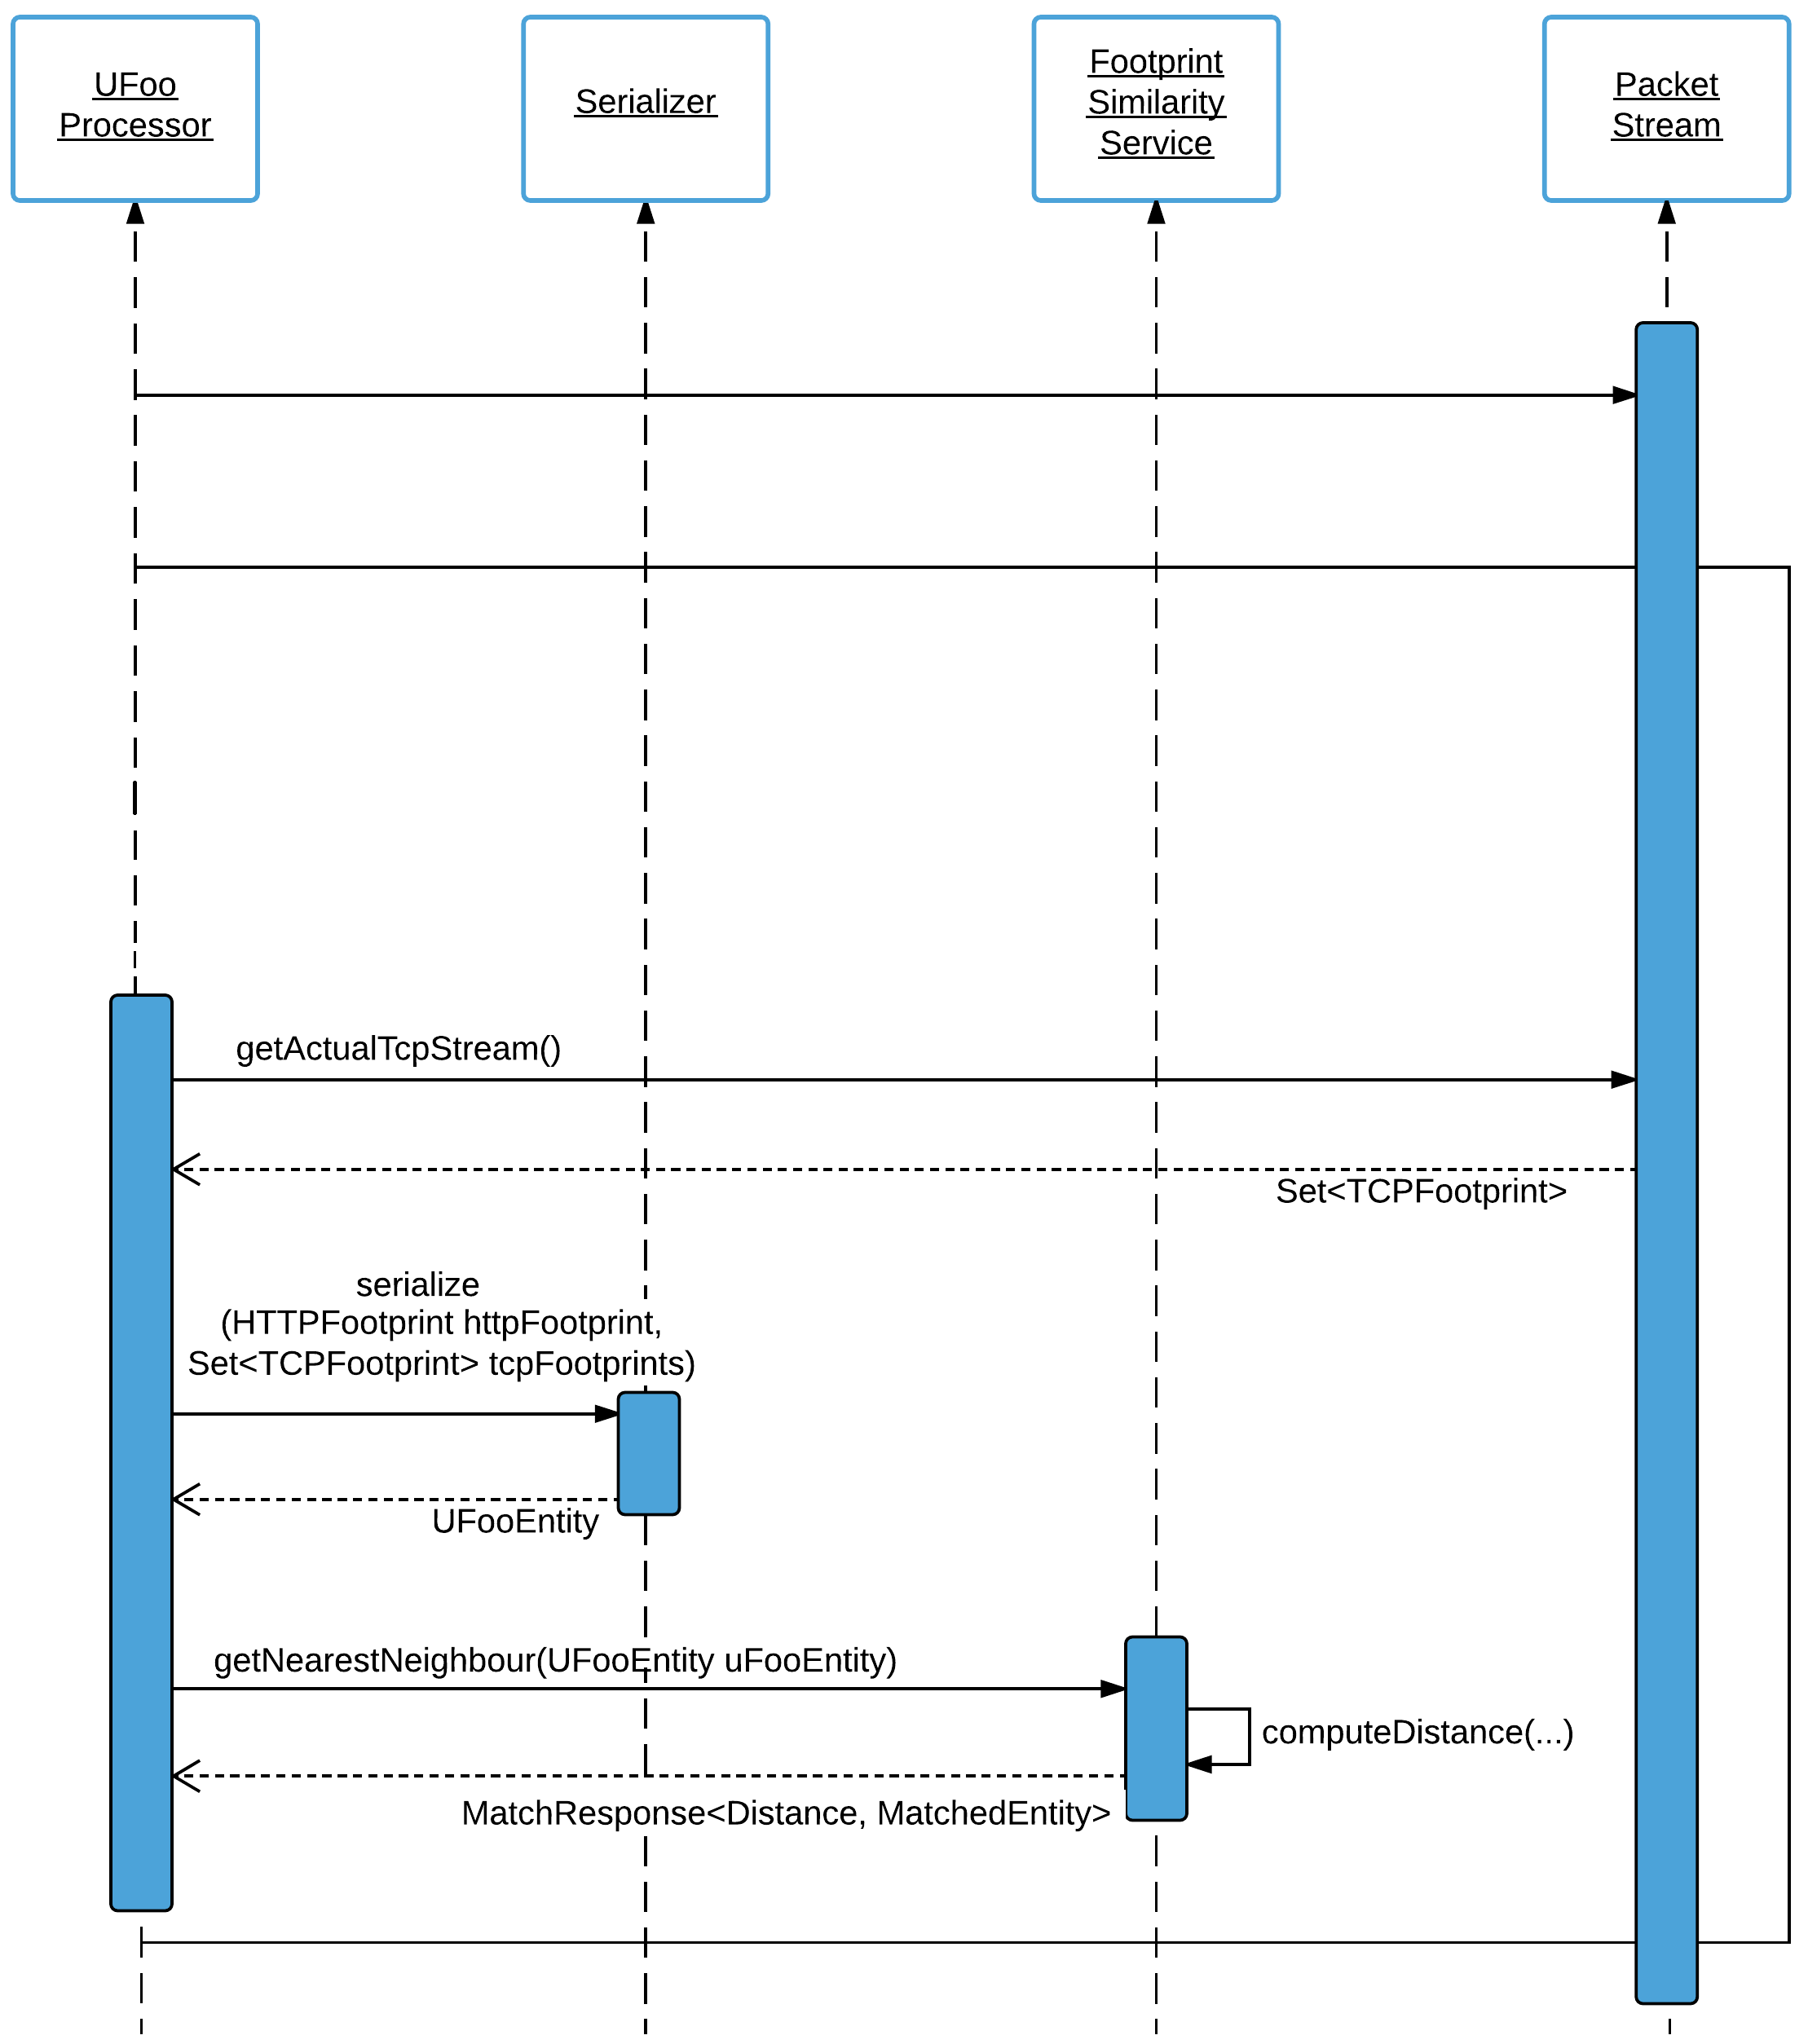
\includegraphics[width=1.1\textwidth]{images/footprint-impl-flow-2.png}
\end{figure}

\chapter{Triedy \textit{HTTPFootprint} a \textit{TCPootprint}}
\label{fig:appendix-structure}
\begin{figure}[h]
  \centering
    
\includegraphics[width=\textwidth]{images/appendix-structure.png}
\end{figure}

%TODO printed
%\chapter{Obsah CD}
%Priložené CD obsahuje nasledujúce adresáre:
%\begin{itemize}
%\item \texttt{dp/thesis} -- obsahuje text bakalárskej práce vo formáte PDF a
%zdrojové soubory vo formáte \LaTeX
%\item \texttt{dp/ufoo} -- obsahuje zdrojový kód implementačnej časti práce,
%teda knižnicu implementujúcu algoritmus identifikácie užívateľa v jazyku Java
%\item \texttt{dp/exampleServer} -- obsahuje spustiteľný JAR súbor aplikácie, v
%ktorej je použitá knižnica implementačnej časti práce, spolu s inštrukciami pre
%jej testovanie
%\end{itemize}
%Aktuálna verzia diplomovej práce, implementácie a jednotlivých príkladov je
%takisto k dispozícií v repozitári \url{https://github.com/m-mato/dp.git}.

\end{document}
